\chapter{Application}

In this section screenshots of the system will be shown. Each screenshot represents different module of system.

\section{Web Application}

The main page of website is shown in Figure \ref{fig:main1}. For now it is only for a demo homepage. Only dynamic functions are register and login for now.There are different login pages for administrators and users. The page they are going to see are different from each other based on their roles.

\begin{figure}[!htbp]
\centering
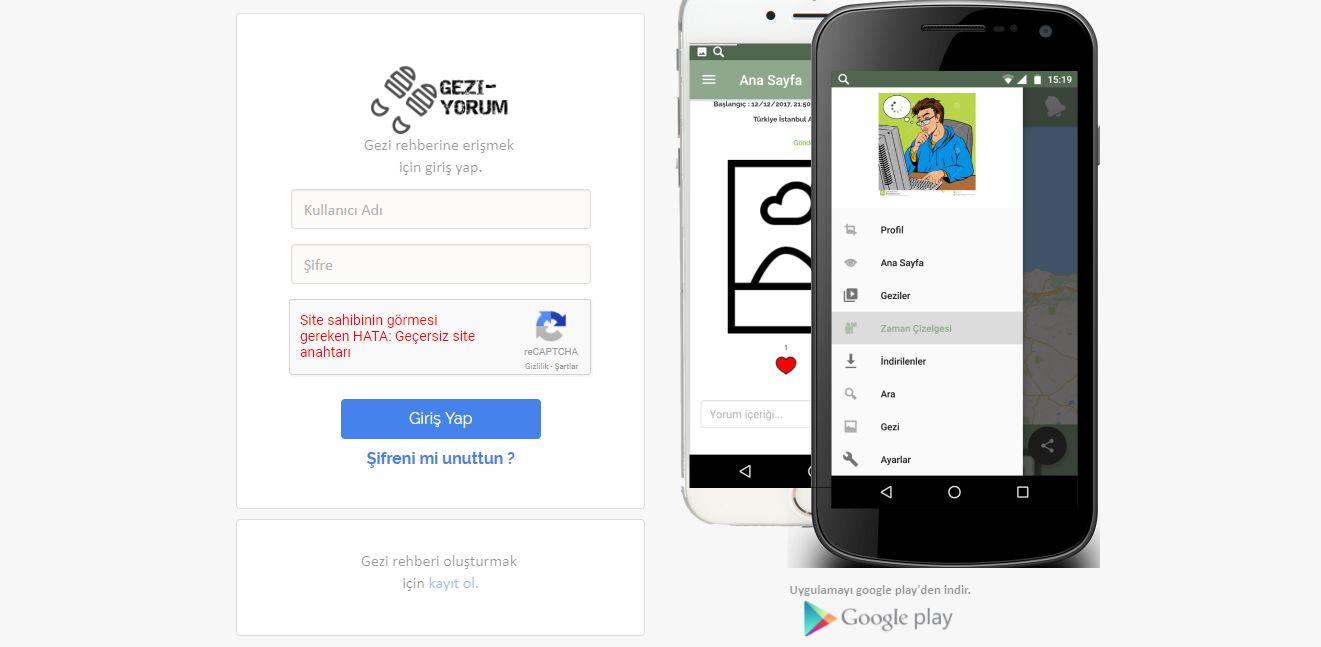
\includegraphics[width=\textwidth]{projectChapters/images/main1.png}
\caption{Main page of the website}
\label{fig:main1}
\end{figure}

\newpage

Users can register from register page by typing their personal information. It is shown in figure  \ref{fig:registerWeb}. 

\begin{figure}[!htbp]
\centering
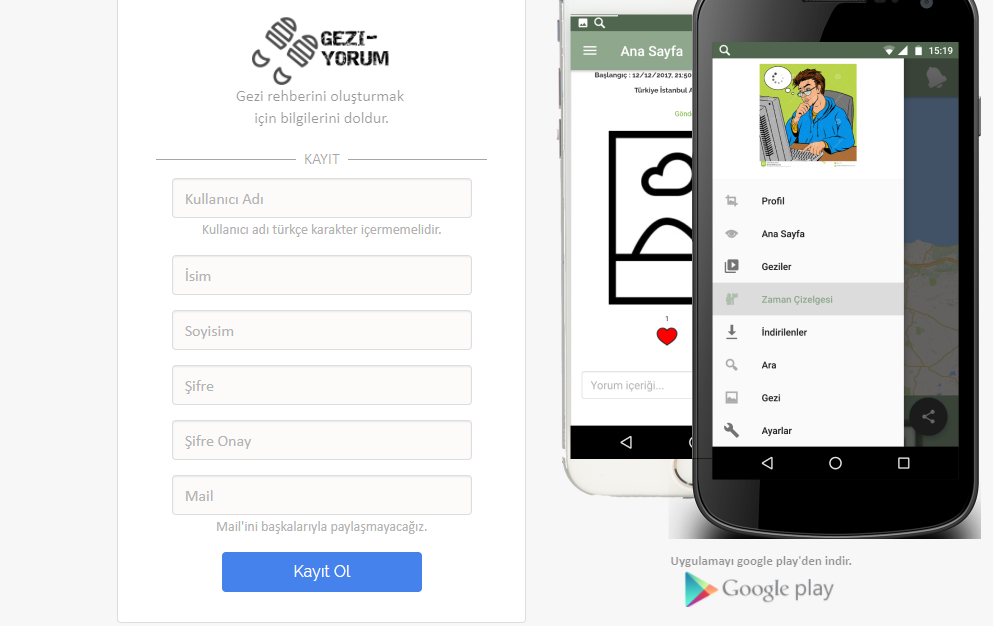
\includegraphics[width=\textwidth]{projectChapters/images/main2.png}
\caption{Register screen for users}
\label{fig:registerWeb}
\end{figure}

\newpage

Users can validate their account by redirecting the address that has been sent to them via our SMTP. It is shown in figure  \ref{fig:registerWeb}. 

\begin{figure}[!htbp]
\centering
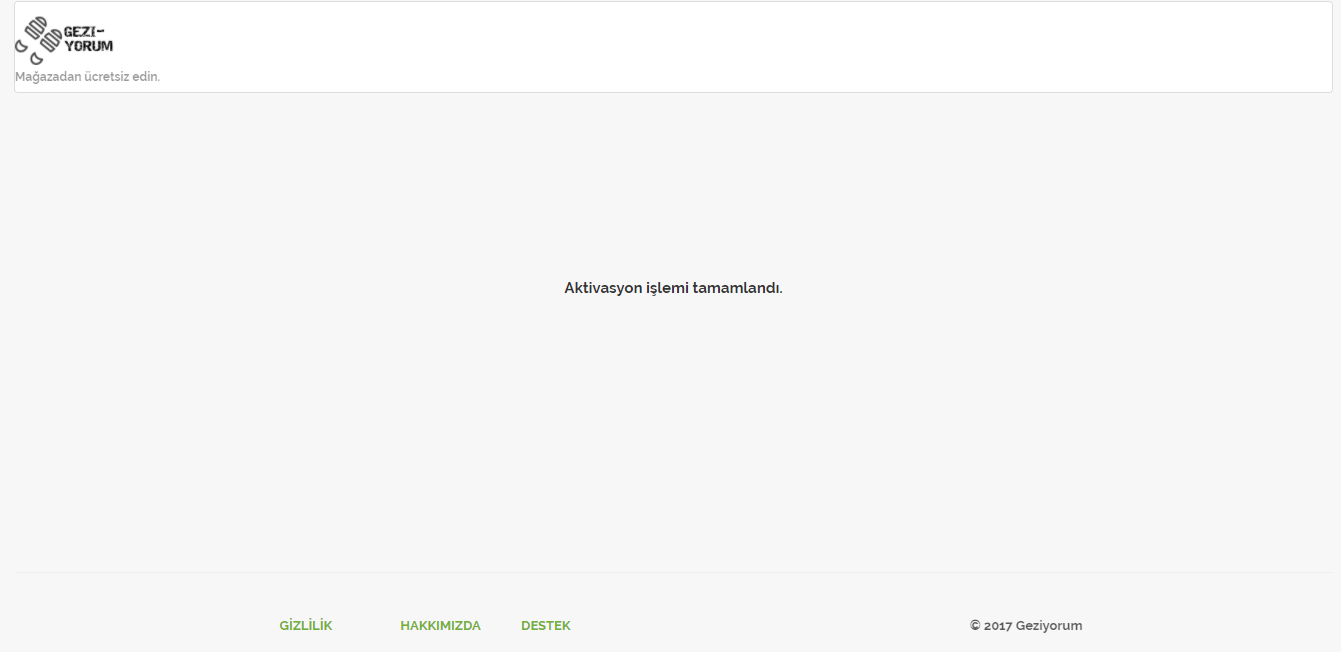
\includegraphics[width=\textwidth]{projectChapters/images/activasion.png}
\caption{Activation screen for users}
\label{fig:registerWeb}
\end{figure}

\newpage

Users can change their account's password by clicking on the forgot password section and filling the username area in the main page, they can change their password by redirecting the address that has been sent to them via our SMTP. It is shown in figure  \ref{fig:registerWeb}. 

\begin{figure}[!htbp]
\centering
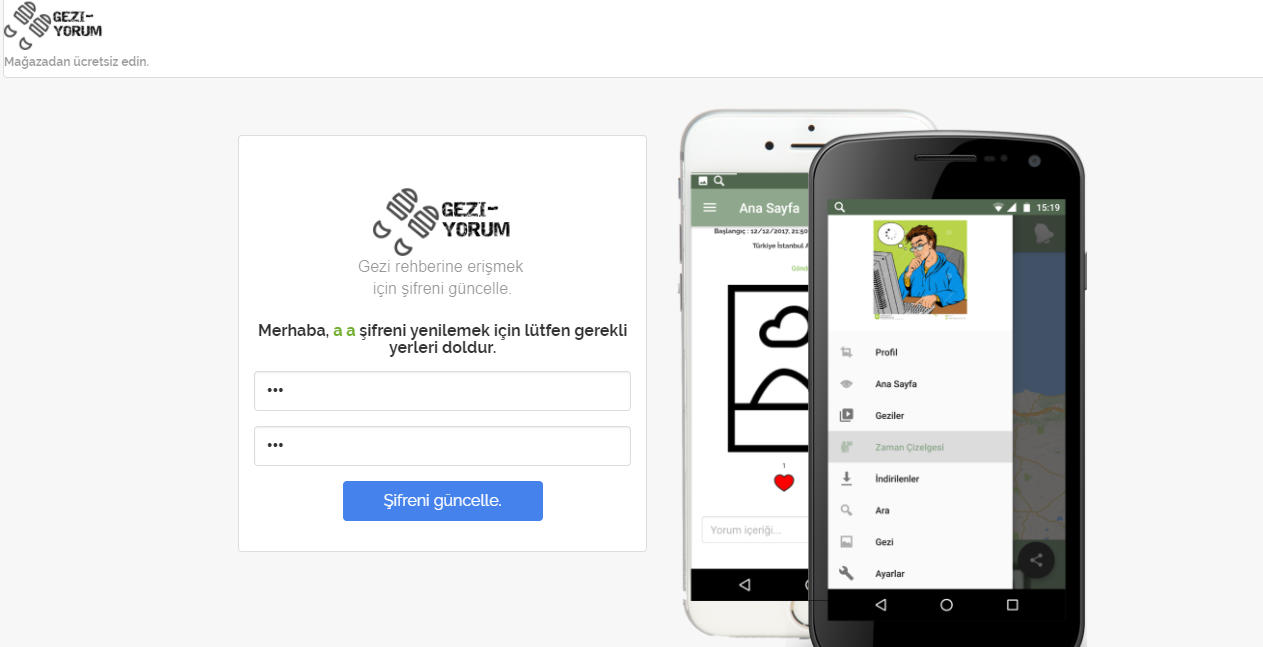
\includegraphics[width=\textwidth]{projectChapters/images/forgetpass.png}
\caption{Forgot my password screen for users}
\label{fig:registerWeb}
\end{figure}





\newpage

Users can access to the developers by using support page, and can read the privacy principles for the permission they are going to give site owners about their usage. It is shown in figure  \ref{fig:supportWeb}. 

\begin{figure}[!htbp]
\centering
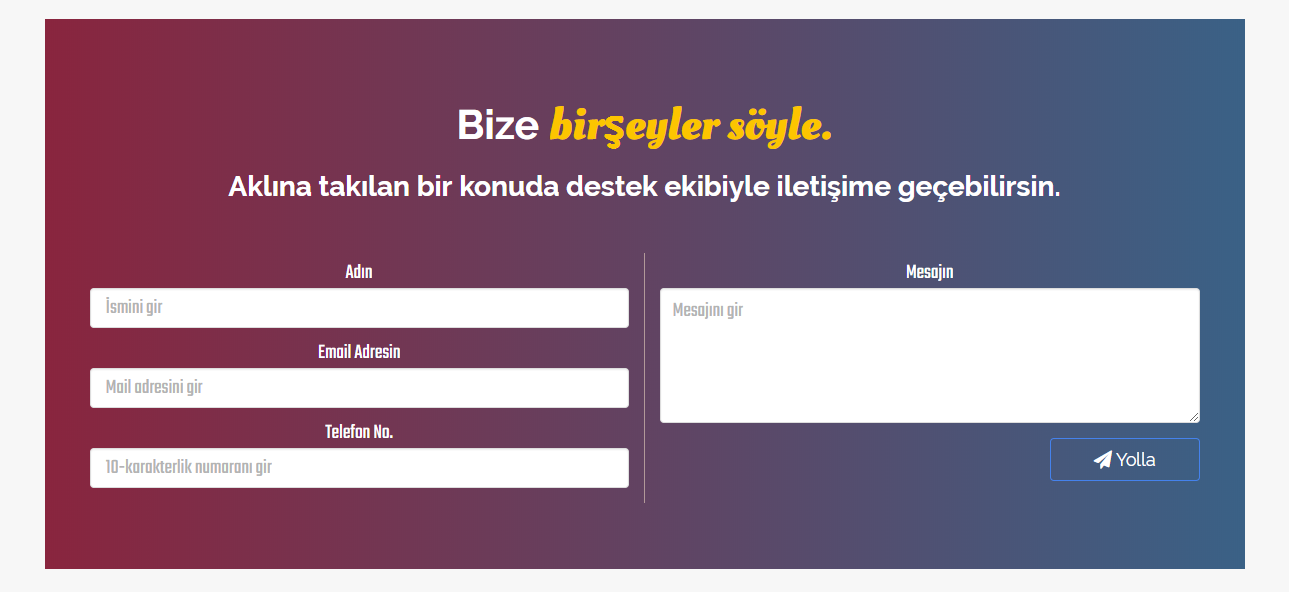
\includegraphics[width=\textwidth]{projectChapters/images/supportPage.png}
\caption{Support screen for users}
\label{fig:supportWeb}
\end{figure}

\newpage

After being logged in users are going to see the home page of website.  It is shown in figure  \ref{fig:homepageWeb}. In this page, users are able to search through the site by typing what they looking for which can be not only users but also trips. It will redirect users to detailed search page afterwards. They can also navigate by using header section of the web page to the their personal profile page and notifications page and detailed search page.

\begin{figure}[!htbp]
\centering
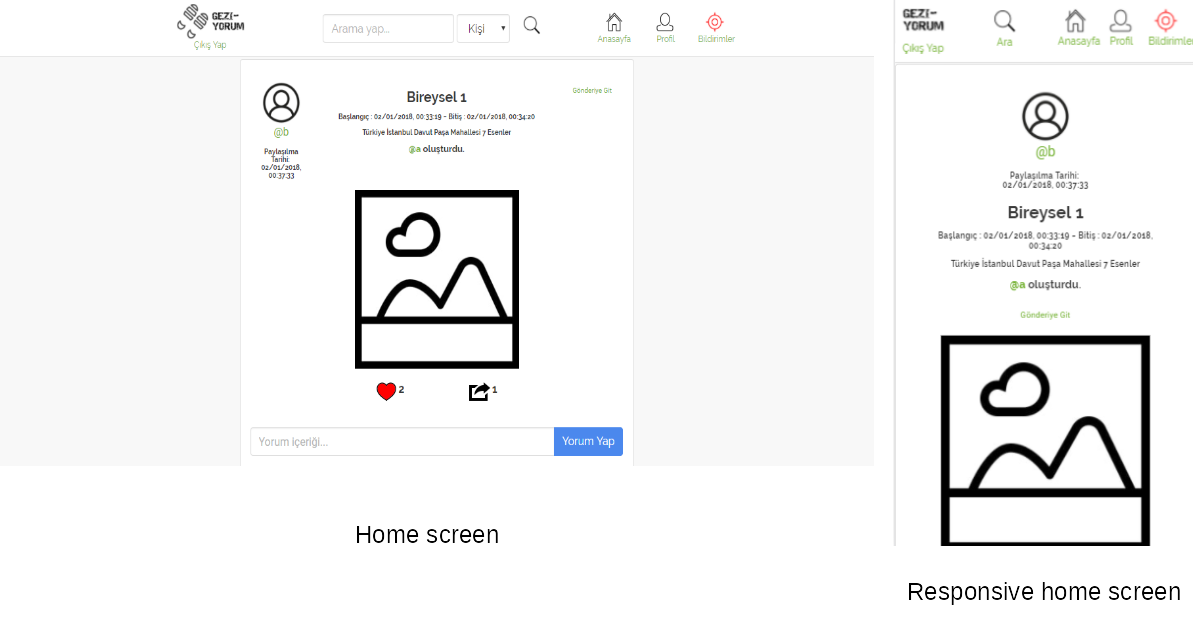
\includegraphics[width=\textwidth]{projectChapters/images/homepageWeb.png}
\caption{Home screen for users}
\label{fig:homepageWeb}
\end{figure}

\newpage

Every page's screen can also turn into dynamic responsive web page no matter what kind of device users use. For example home pages responsive screen is shown in Figure  \ref{fig:homepageRespon}.

\begin{figure}[!htbp]
\centering
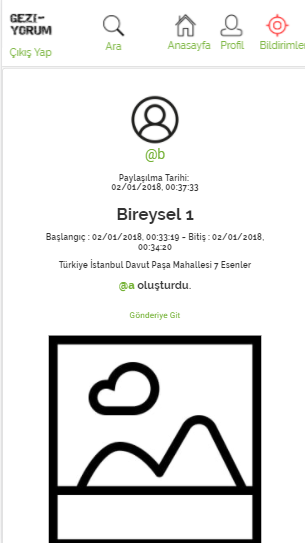
\includegraphics[width=50mm,scale=0.5]{projectChapters/images/homepageResponsive.png}
\caption{Responsive home screen for users}
\label{fig:homepageRespon}
\end{figure}

\newpage

Web page has a notification page which contains users interaction informations. When an user comments on other users trip the other user will be informed by using this screen he or she can hide as he or she prefer, also friend requests can be seen from this screen. Users can accept or deny these requests. The screen is shown in Figure  \ref{fig:notificationPage}.

\begin{figure}[!htbp]
\centering
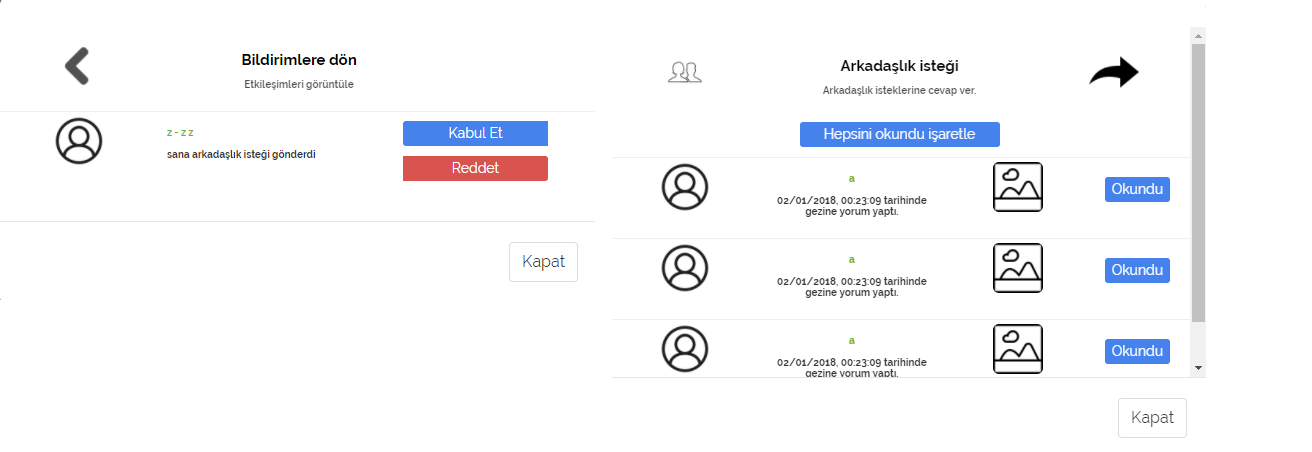
\includegraphics[width=\textwidth]{projectChapters/images/notificationPage.png}
\caption{Notification screen for users}
\label{fig:notificationPage}
\end{figure}


\newpage

Users are able to see their personal screen through the profile page. It contains their personal trips list and the ones they shared. Also they can see their friends list they can also unfriend them if they want. The screen is shown in Figure  \ref{fig:profileWeb1}.

\begin{figure}[!htbp]
\centering
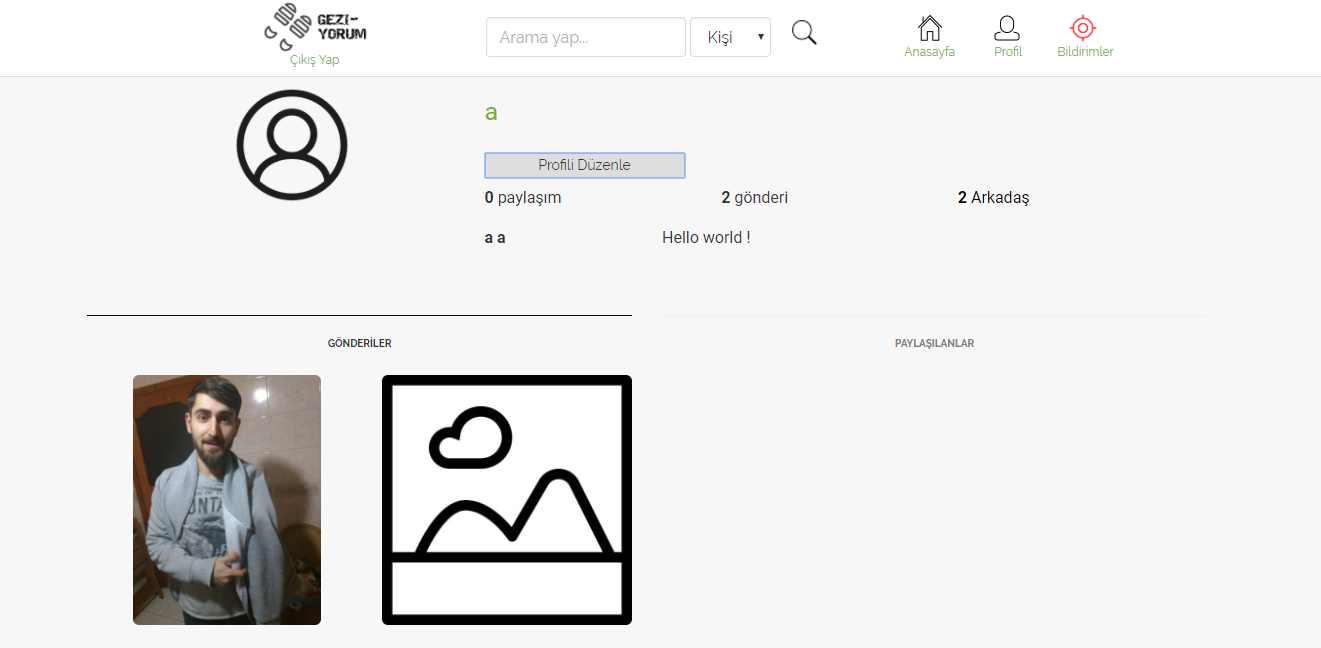
\includegraphics[width=\textwidth]{projectChapters/images/profileWeb1.png}
\caption{Profile page for users}
\label{fig:profileWeb1}
\end{figure}

\newpage

Users can see their personal informations such as name, surname, e-mail, website and so on and they can change them if they want. The screen is shown in Figure  \ref{fig:profileWeb2}.

\begin{figure}[!htbp]
\centering
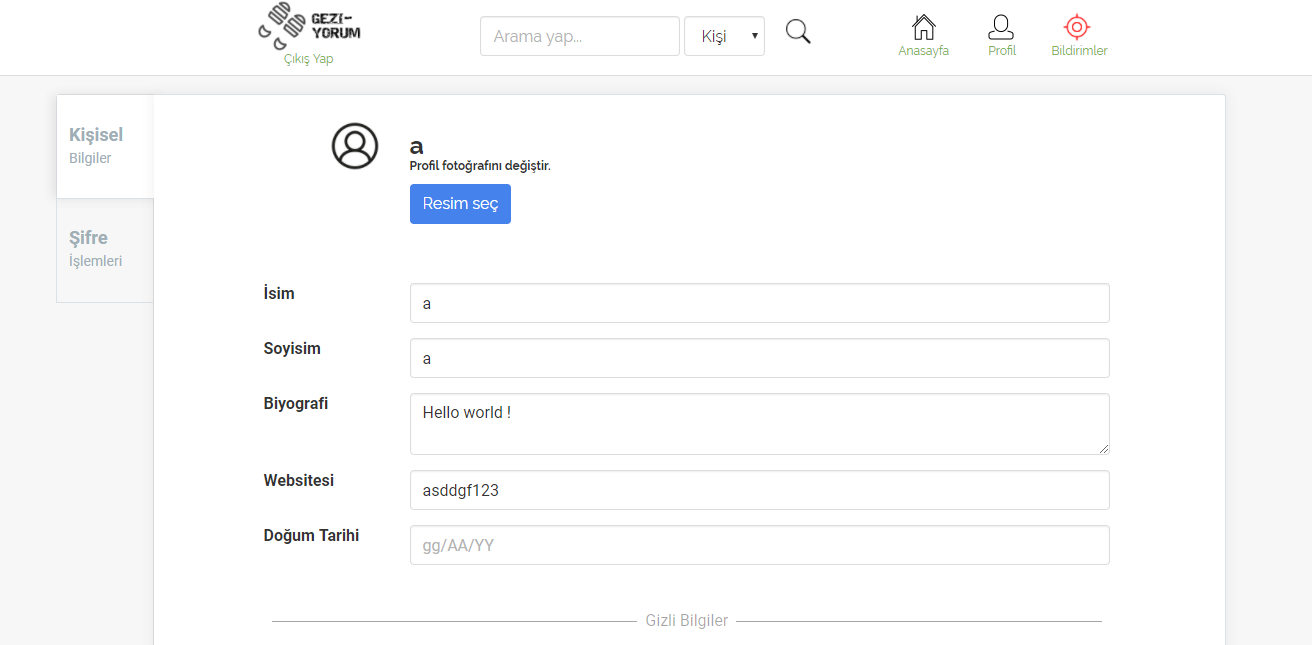
\includegraphics[width=\textwidth]{projectChapters/images/profileWeb2.png}
\caption{Profile page for users}
\label{fig:profileWeb2}
\end{figure}

\newpage

Users can change their password and upload profile picture from this page. The page is shown in Figure  \ref{fig:profileWeb3}.

\begin{figure}[!htbp]
\centering
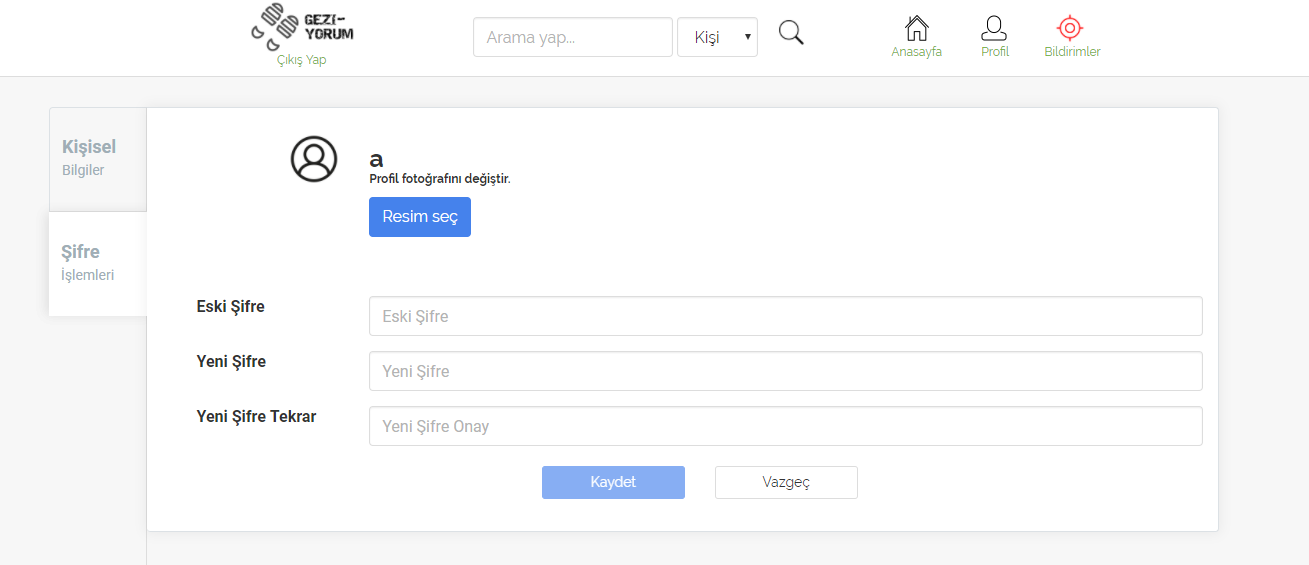
\includegraphics[width=\textwidth]{projectChapters/images/profileWeb3.png}
\caption{Profile page for users}
\label{fig:profileWeb3}
\end{figure}

\newpage

Other users page can be seen through the users page they can send friend requests by using this page, also if they think the owner of the page have some inappropriate content they can create a complaint. The page is shown in Figure   \ref{fig:userpageWeb}.

\begin{figure}[!htbp]
\centering
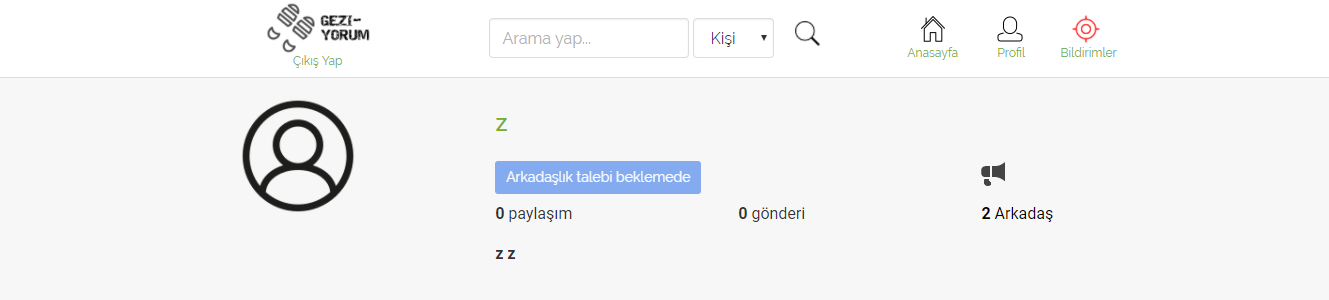
\includegraphics[width=\textwidth]{projectChapters/images/userpageWeb.png}
\caption{User page}
\label{fig:userpageWeb}
\end{figure}

\newpage

Users can create complaints about profiles, shared trips or comments if they think the contents of them contains some harmful information, harassments or insulting. The page is shown in Figure \ref{fig:complaintPage}. 

\begin{figure}[!htbp]
\centering
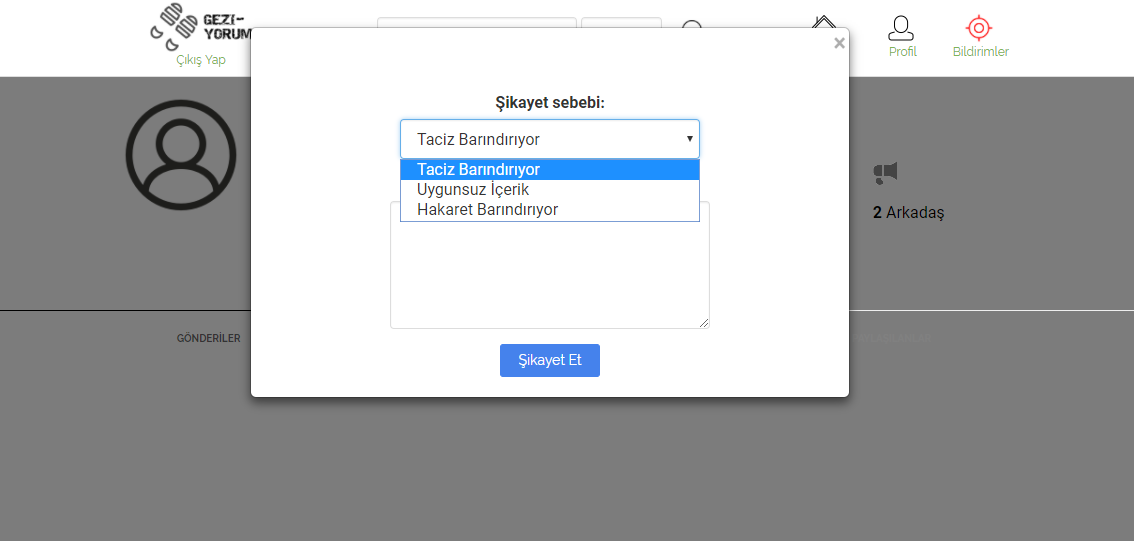
\includegraphics[width=\textwidth]{projectChapters/images/complaintPage.png}
\caption{Creating complaint screen for users, trips and comments}
\label{fig:complaintPage}
\end{figure}

\newpage

Trips details can be seen by clicking on the trips cover photos. Its detailed screen contains information about where it is happened, persons who participated, the owner of it, what time it is created, the medias and the comments of medias, comments which the other users writed. It also contains like and share buttons, and writing comment section, lastly complaint creating buttons for both the trip itself and the comments. 
\ref{fig:tripDetail}. 

\begin{figure}[!htbp]
\centering
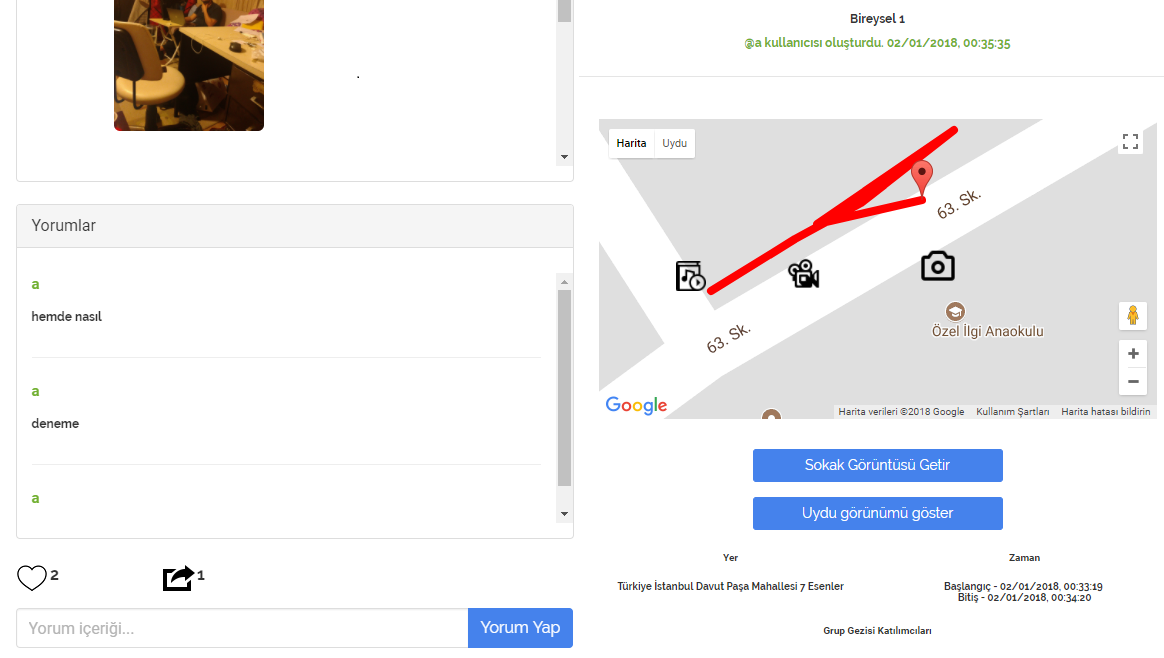
\includegraphics[width=\textwidth]{projectChapters/images/tripDetail.png}
\caption{Trip details screen}
\label{fig:tripDetail}
\end{figure}

\newpage

Users can search trips, users from the search page they can also filter the searching by selecting what type of trip they looking for. They can also choose if they want to see trips   created only by their friends or by any one on the site. The page is shown in Figure   \ref{fig:searchPageWeb}.

\begin{figure}[!htbp]
\centering
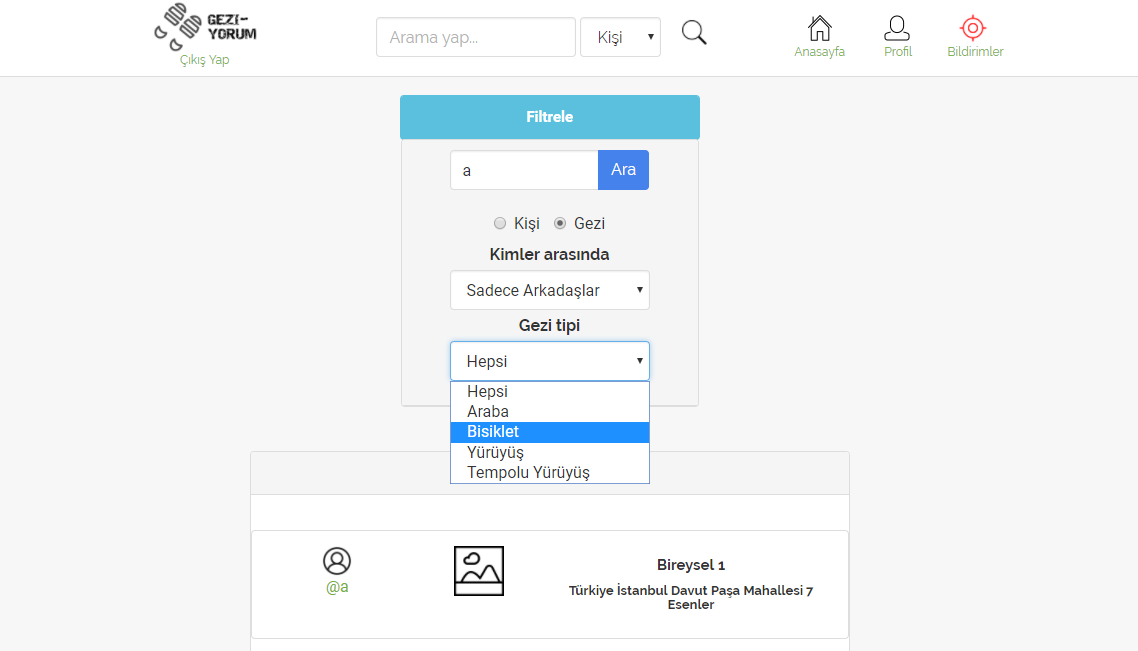
\includegraphics[width=\textwidth]{projectChapters/images/searchPageWeb.png}
\caption{Search page}
\label{fig:searchPageWeb}
\end{figure}

\newpage

We have administrators management page. In this page administrators can see complaints related with users, trips and comments that are created by users. They can see, search, evaluate and list them with this screen which is shown in Figure \ref{fig:admin1}.
\begin{figure}[!htbp]
\centering
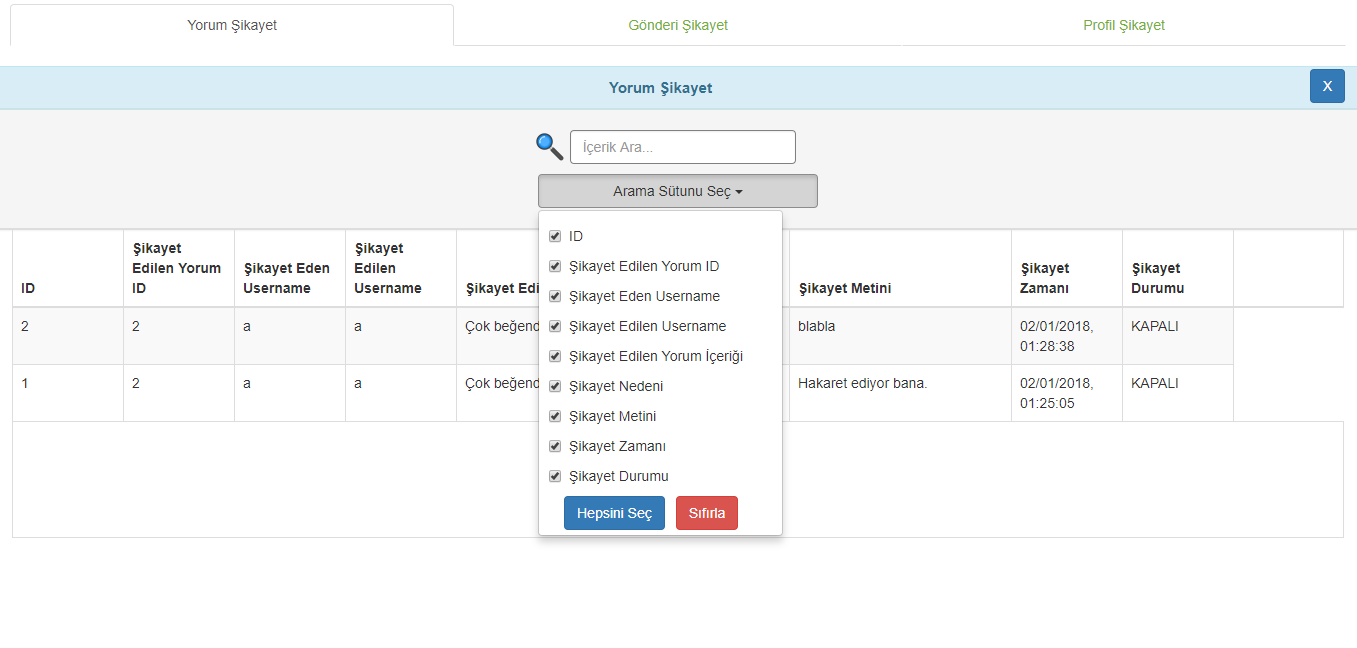
\includegraphics[width=\textwidth]{projectChapters/images/admin1.png}
\caption{Administrator page}
\label{fig:admin1}
\end{figure}

\newpage

Administrators can decide whether the content is going to be hidden or not, we have a screen to decide hide the content or not, which is shown in Figure  \ref{fig:admin2}.

\begin{figure}[!htbp]
\centering
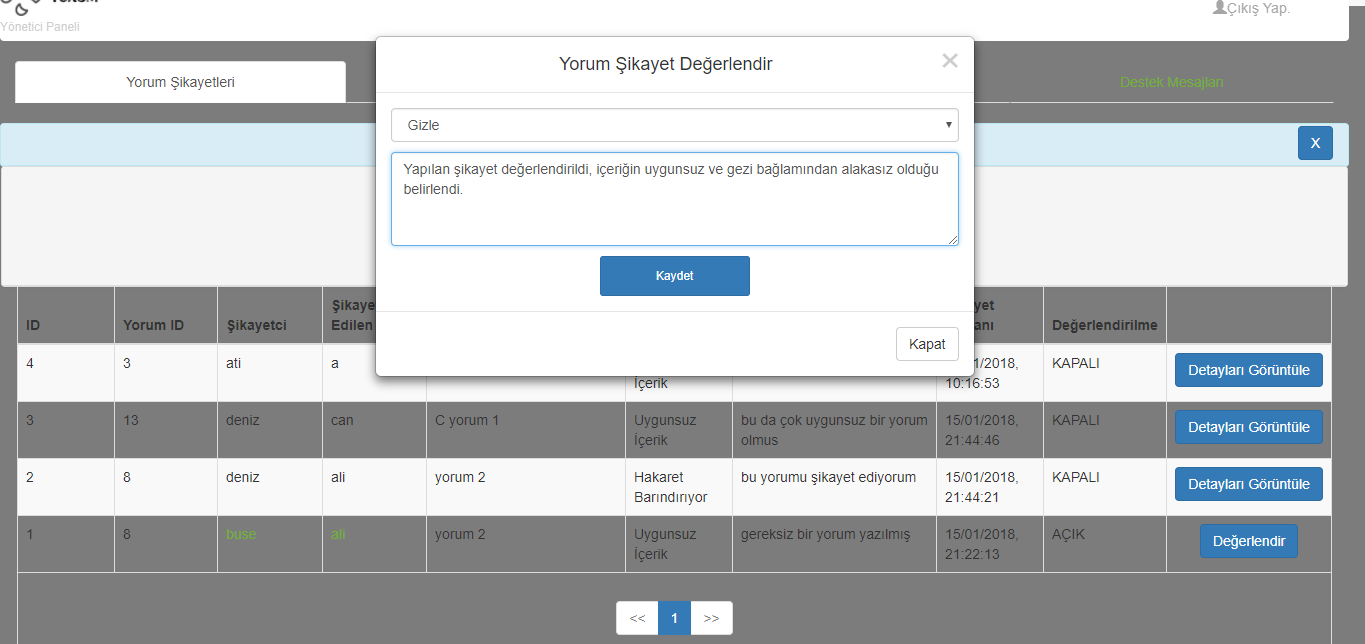
\includegraphics[width=\textwidth]{projectChapters/images/admin2.png}
\caption{Administrator page}
\label{fig:admin2}
\end{figure}

\newpage


\section{Mobile Apllication}

Our application has a mobile side also. Users can login through mobile application to create, share and look for trips. It also contains the web application's every functionalities. Details of mobile application can be seen figures below.

The mobile application has register screen for users, users can register by using this screen which shown in Figure \ref{fig:phoneRegister}.

\begin{figure}[!htbp]
\centering
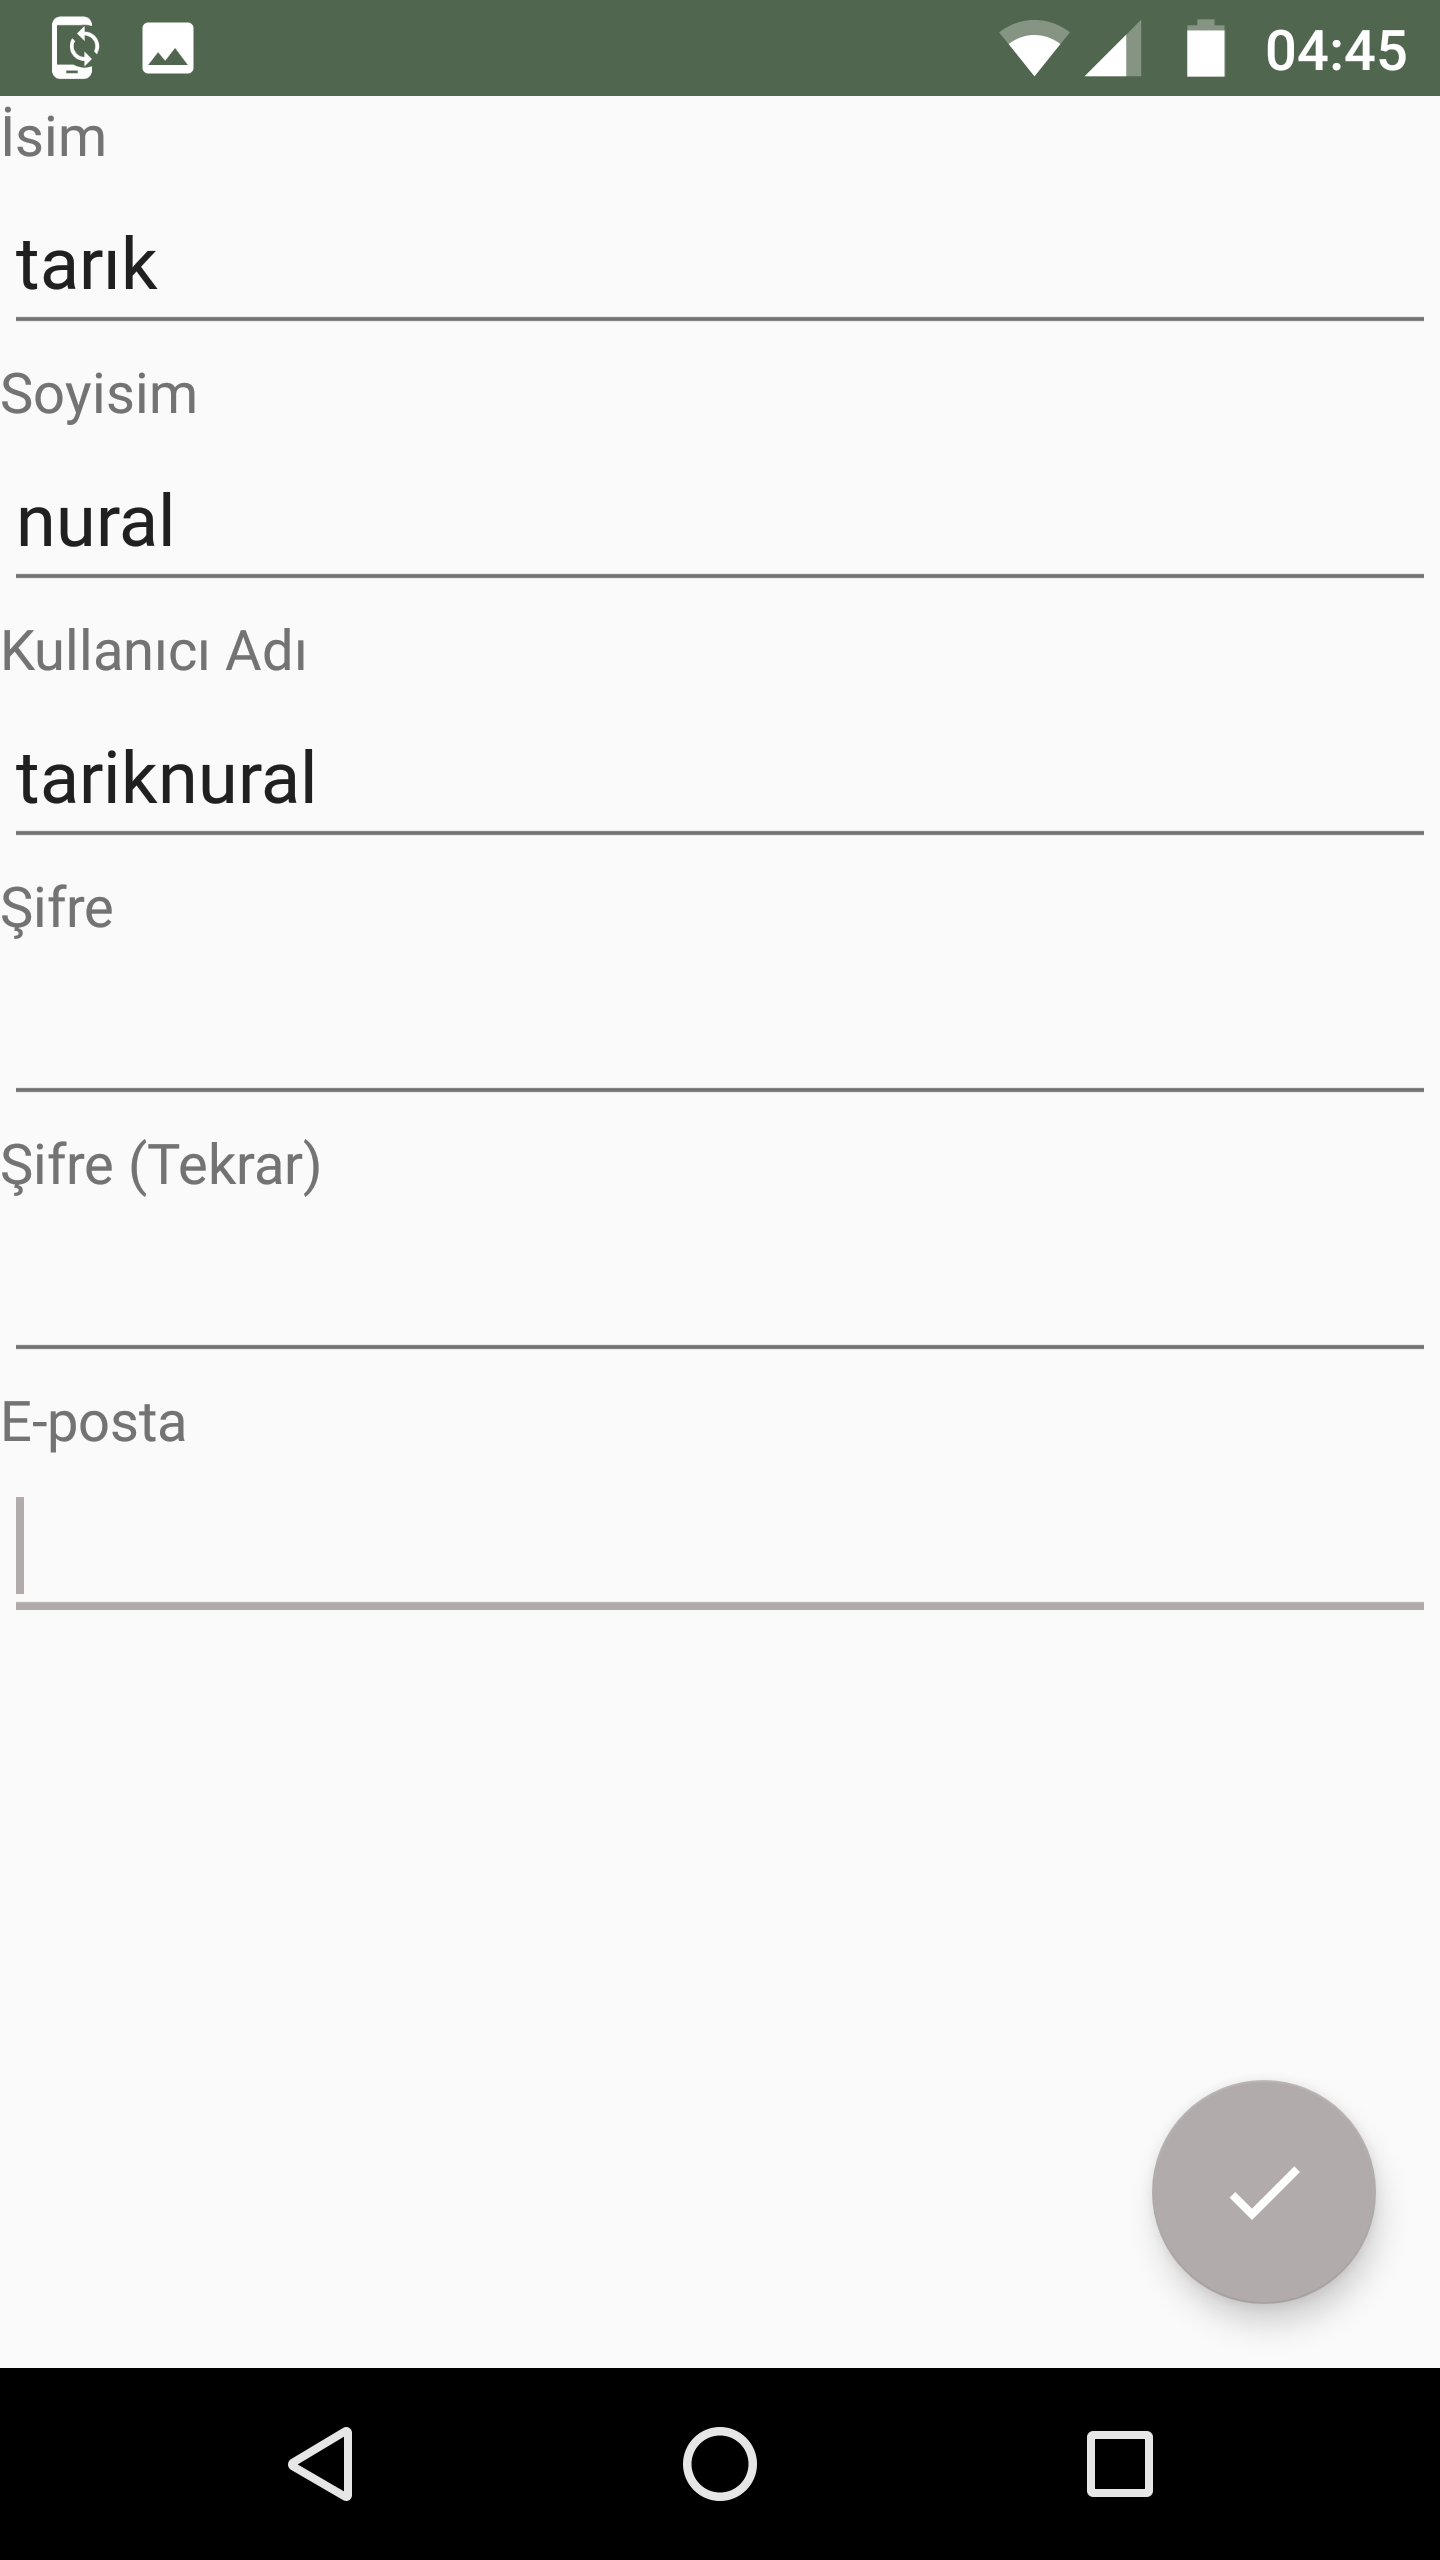
\includegraphics[width=50mm,scale=0.5]{projectChapters/images/phoneRegister.png}
\caption{Mobile application register page}
\label{fig:phoneRegister}
\end{figure}

\newpage

The mobile application has log-in screen for users, without logged in users are not able to use functionalities of creating trips or interact with other users, the screen is shown in Figure \ref{fig:phoneLogin}.  
\begin{figure}[!htbp]
\centering
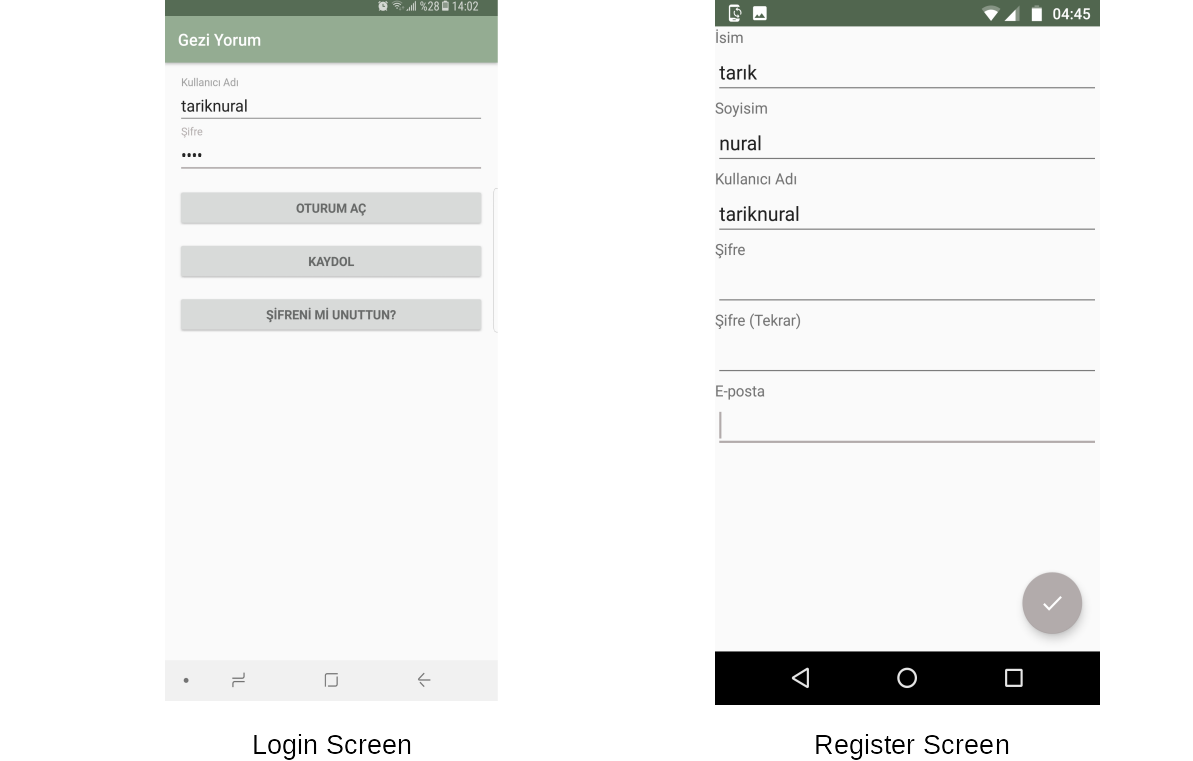
\includegraphics[width=60mm,scale=0.6]{projectChapters/images/phoneLogin.png}
\caption{Mobile application login page}
\label{fig:phoneLogin}
\end{figure}

\newpage

Mobile application has a main section, this page is similar to the web application home page. In this section, users are able to see their friends shared or created trips listed in here.  
\ref{fig:phoneHome}.

\begin{figure}[!htbp]
\centering
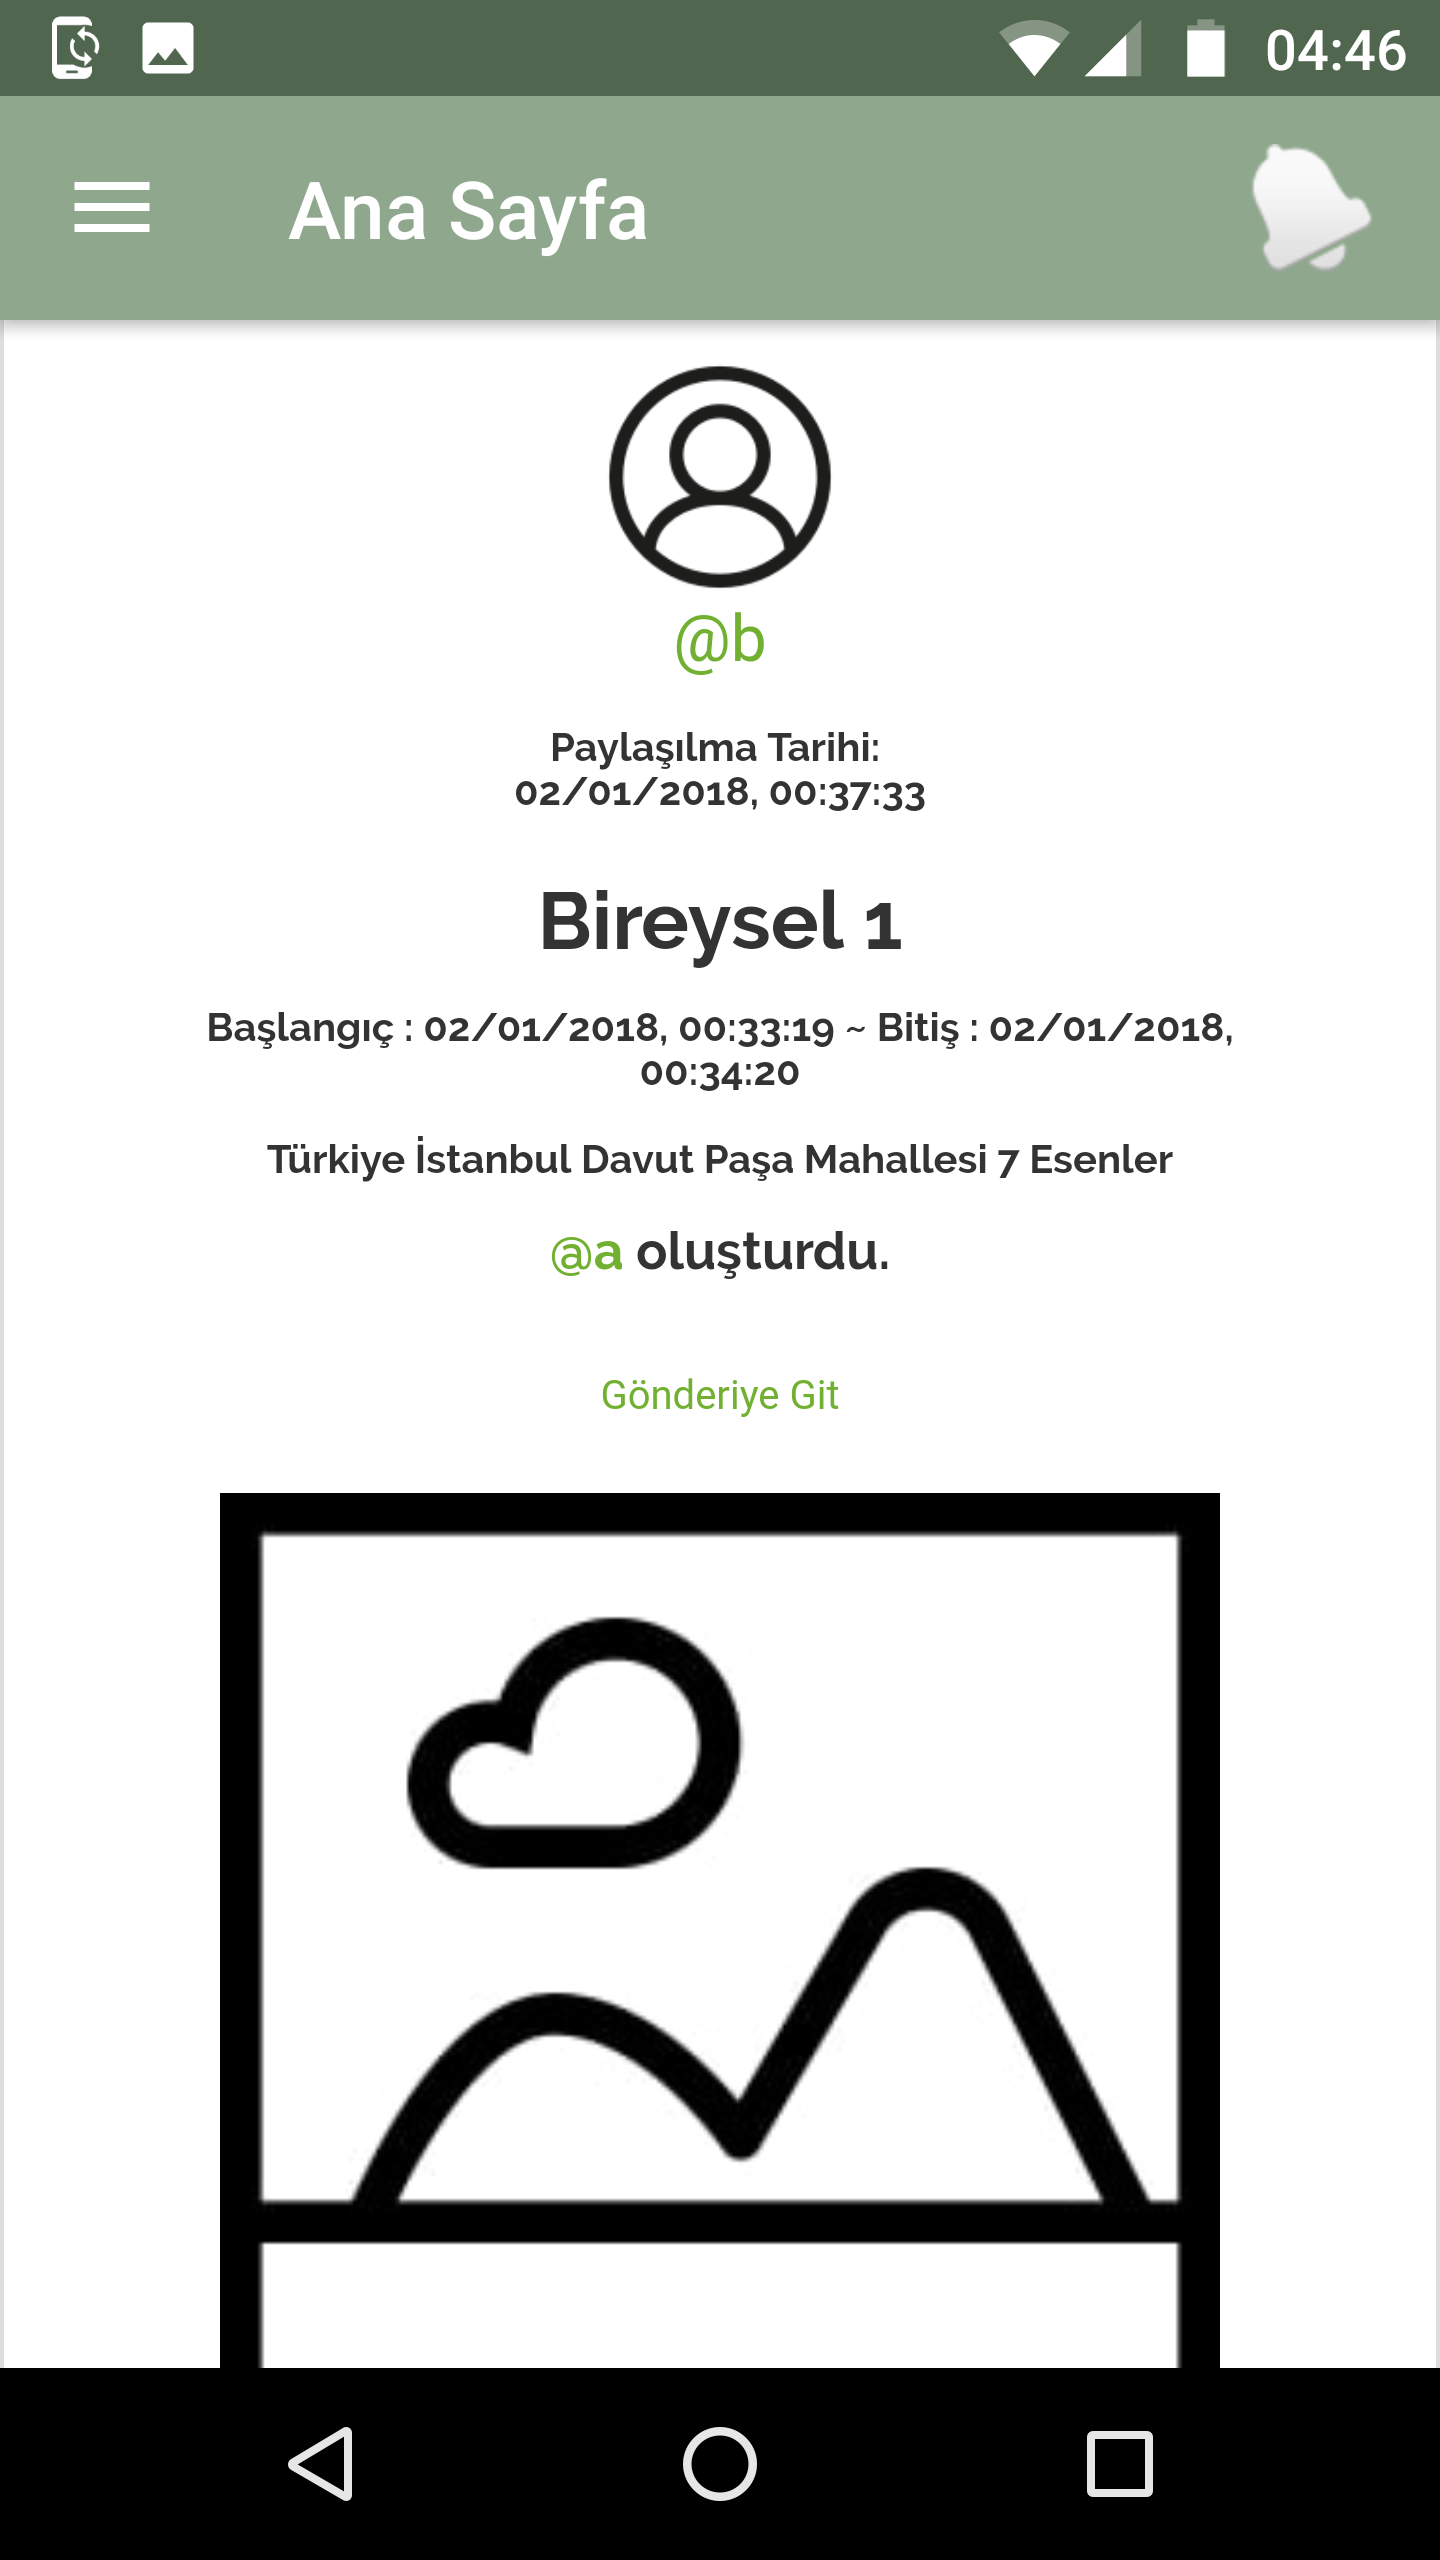
\includegraphics[width=70mm,scale=0.7]{projectChapters/images/phoneHome.png}
\caption{Mobile application home page}
\label{fig:phoneHome}
\end{figure}

\newpage

Mobile application has a notification section which includes friend requests and trip invitation requests. Users can accept or deny those requests in here.
\ref{fig:notificationMobile}.

\begin{figure}[!htbp]
\centering
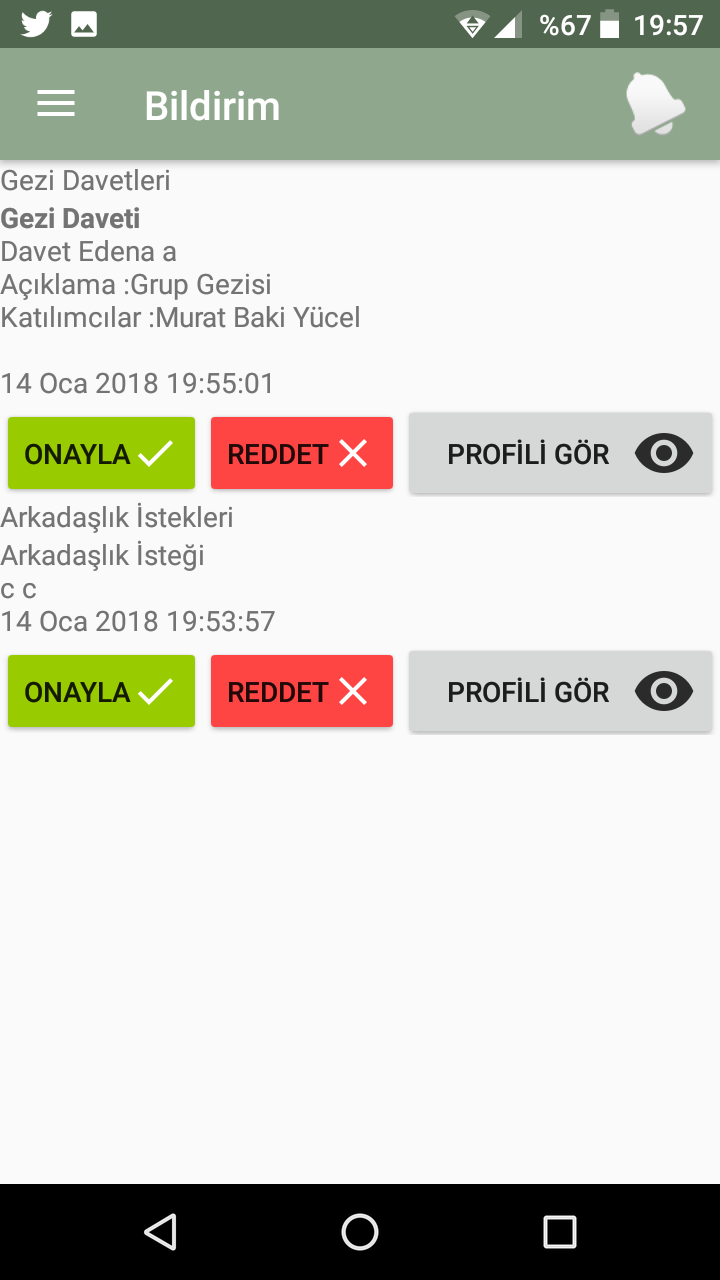
\includegraphics[width=70mm,scale=0.7]{projectChapters/images/notificationMobile.png}
\caption{Mobile application notification page}
\label{fig:notificationMobile}
\end{figure}

\newpage

Mobile application has a profile section, users are able to see their personal screen through the profile page. It contains their personal trips list and the ones they shared. Also they can see their friends list they can also unfriend them if they want. It has same functionalities as web application's profile page. The screen is shown in Figure 
\ref{fig:profileMobile}.

\begin{figure}[!htbp]
\centering
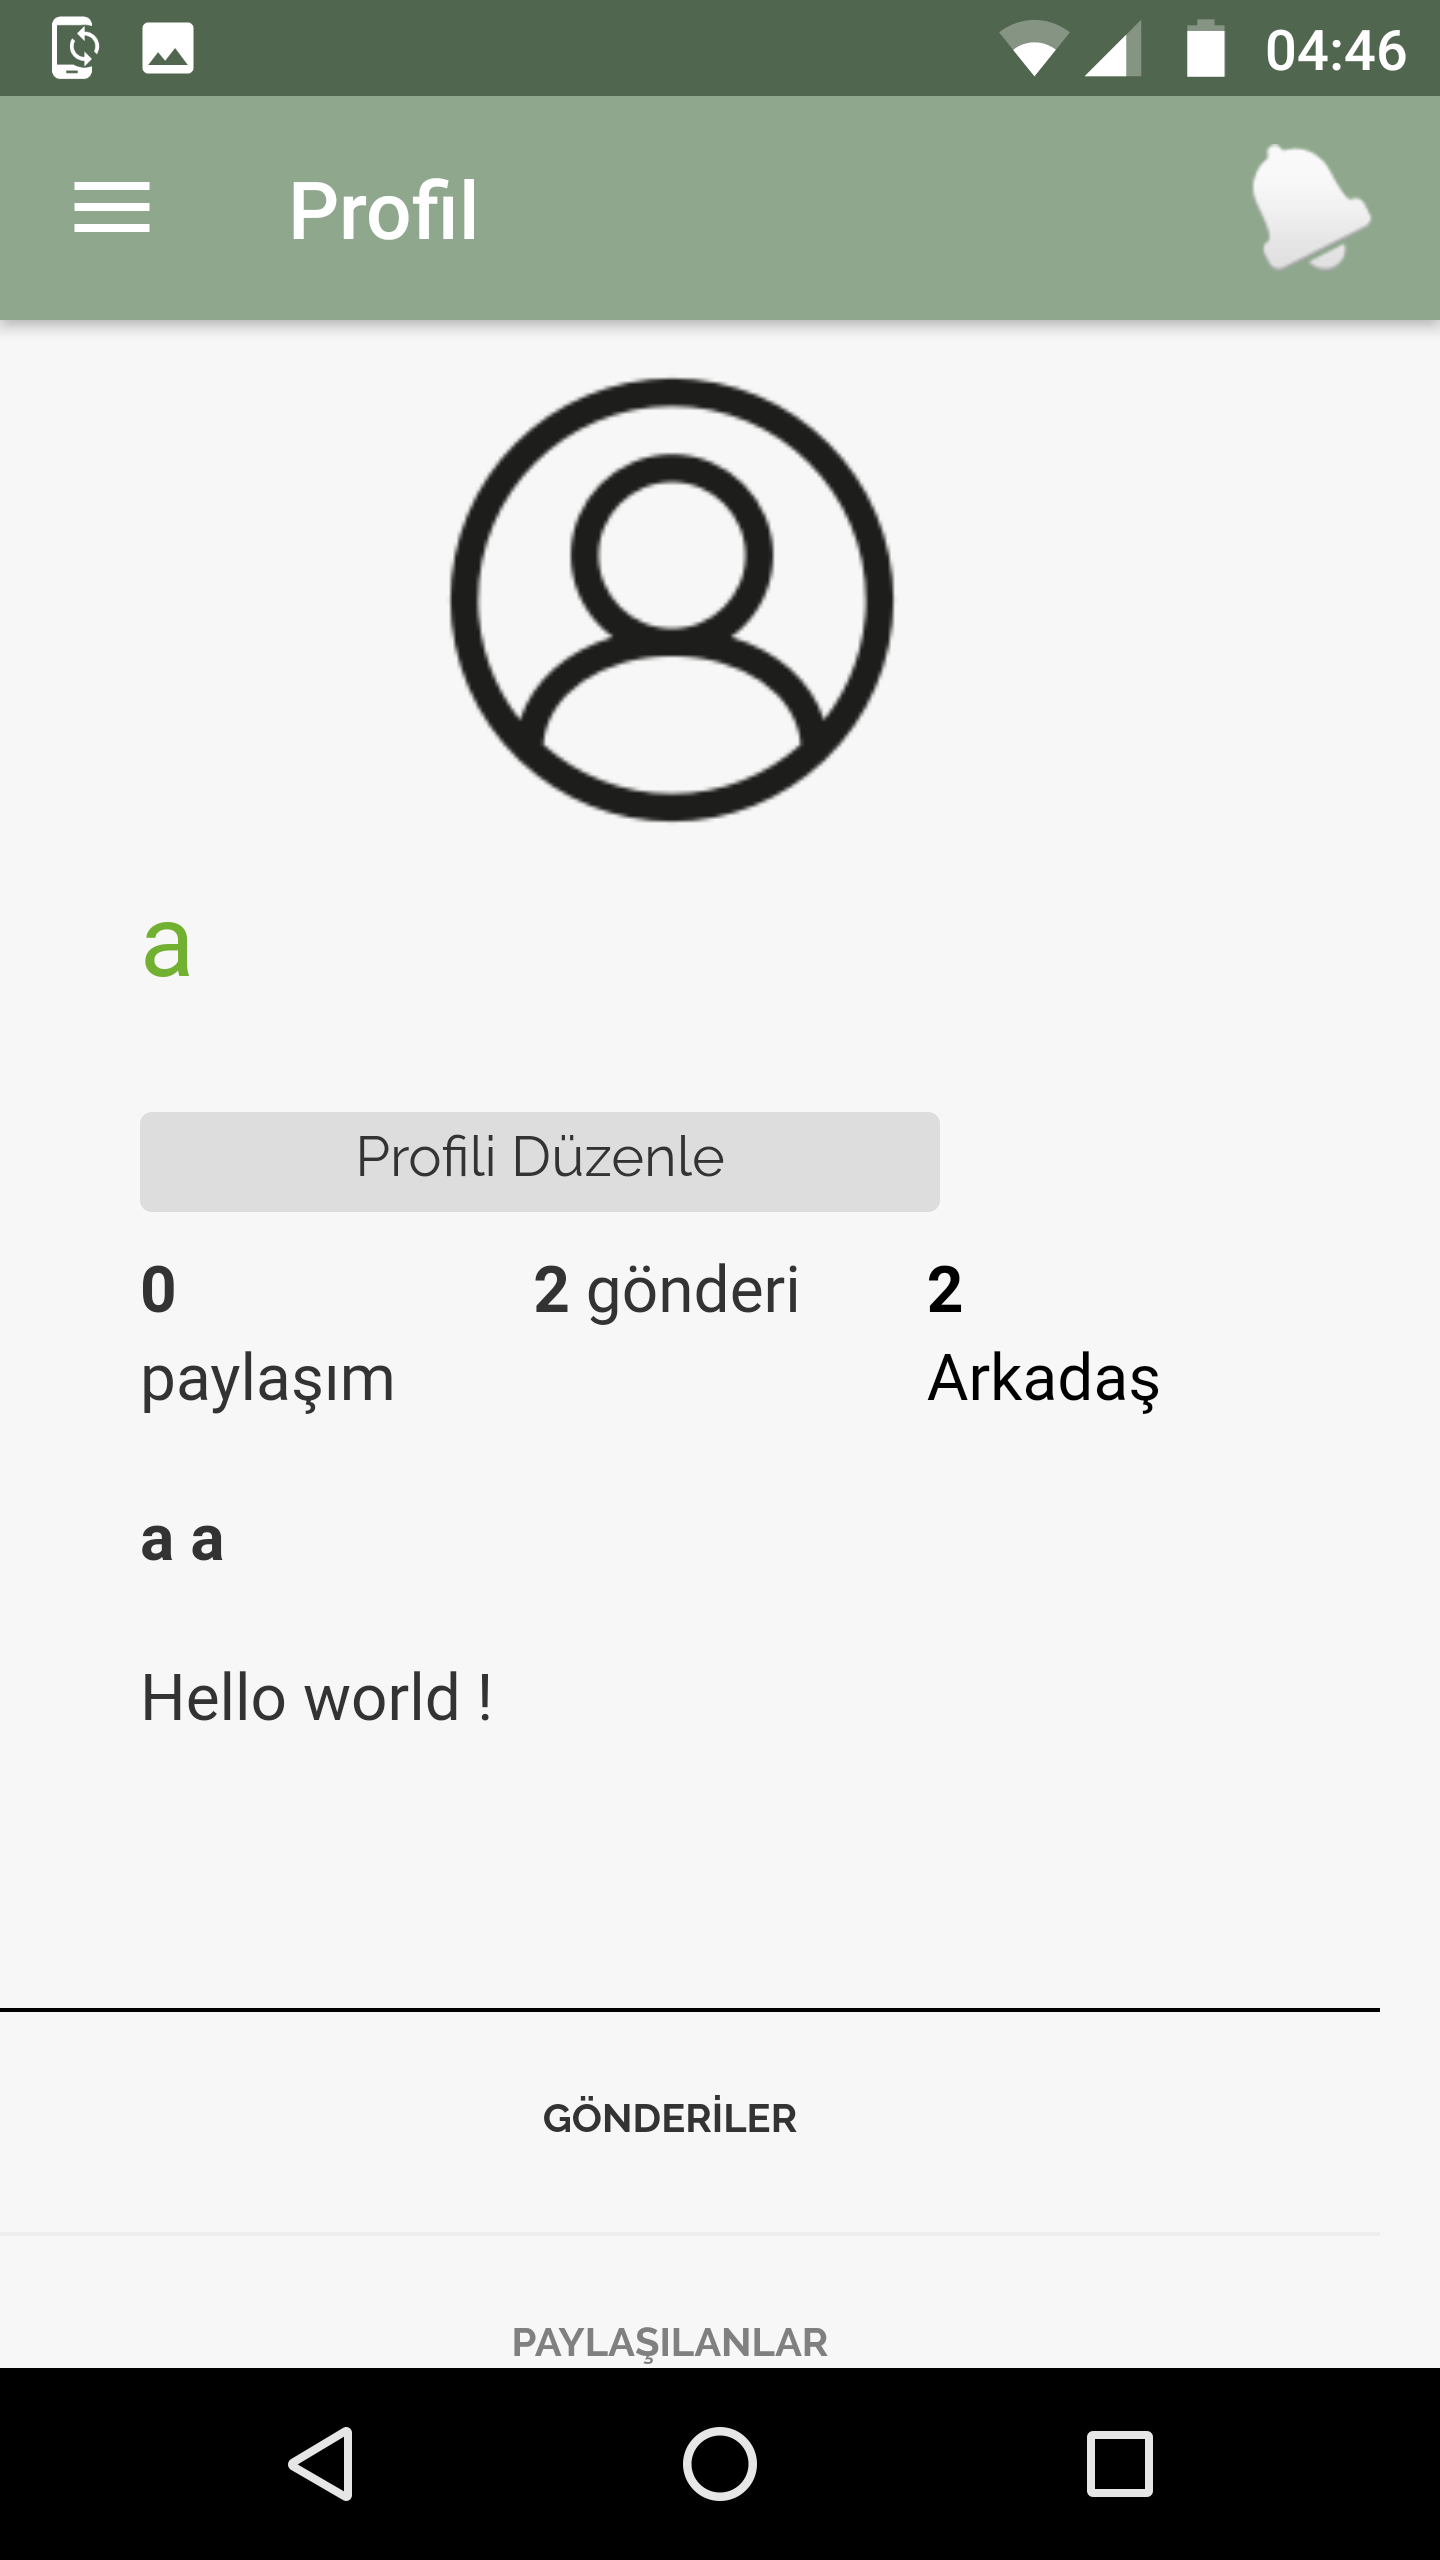
\includegraphics[width=70mm,scale=0.7]{projectChapters/images/profileMobile.png}
\caption{Mobile application profile page}
\label{fig:profileMobile}
\end{figure}

\newpage

Mobile application has trip search module it is same as web application.
\ref{fig:mobilGeziArama}.

\begin{figure}[!htbp]
\centering
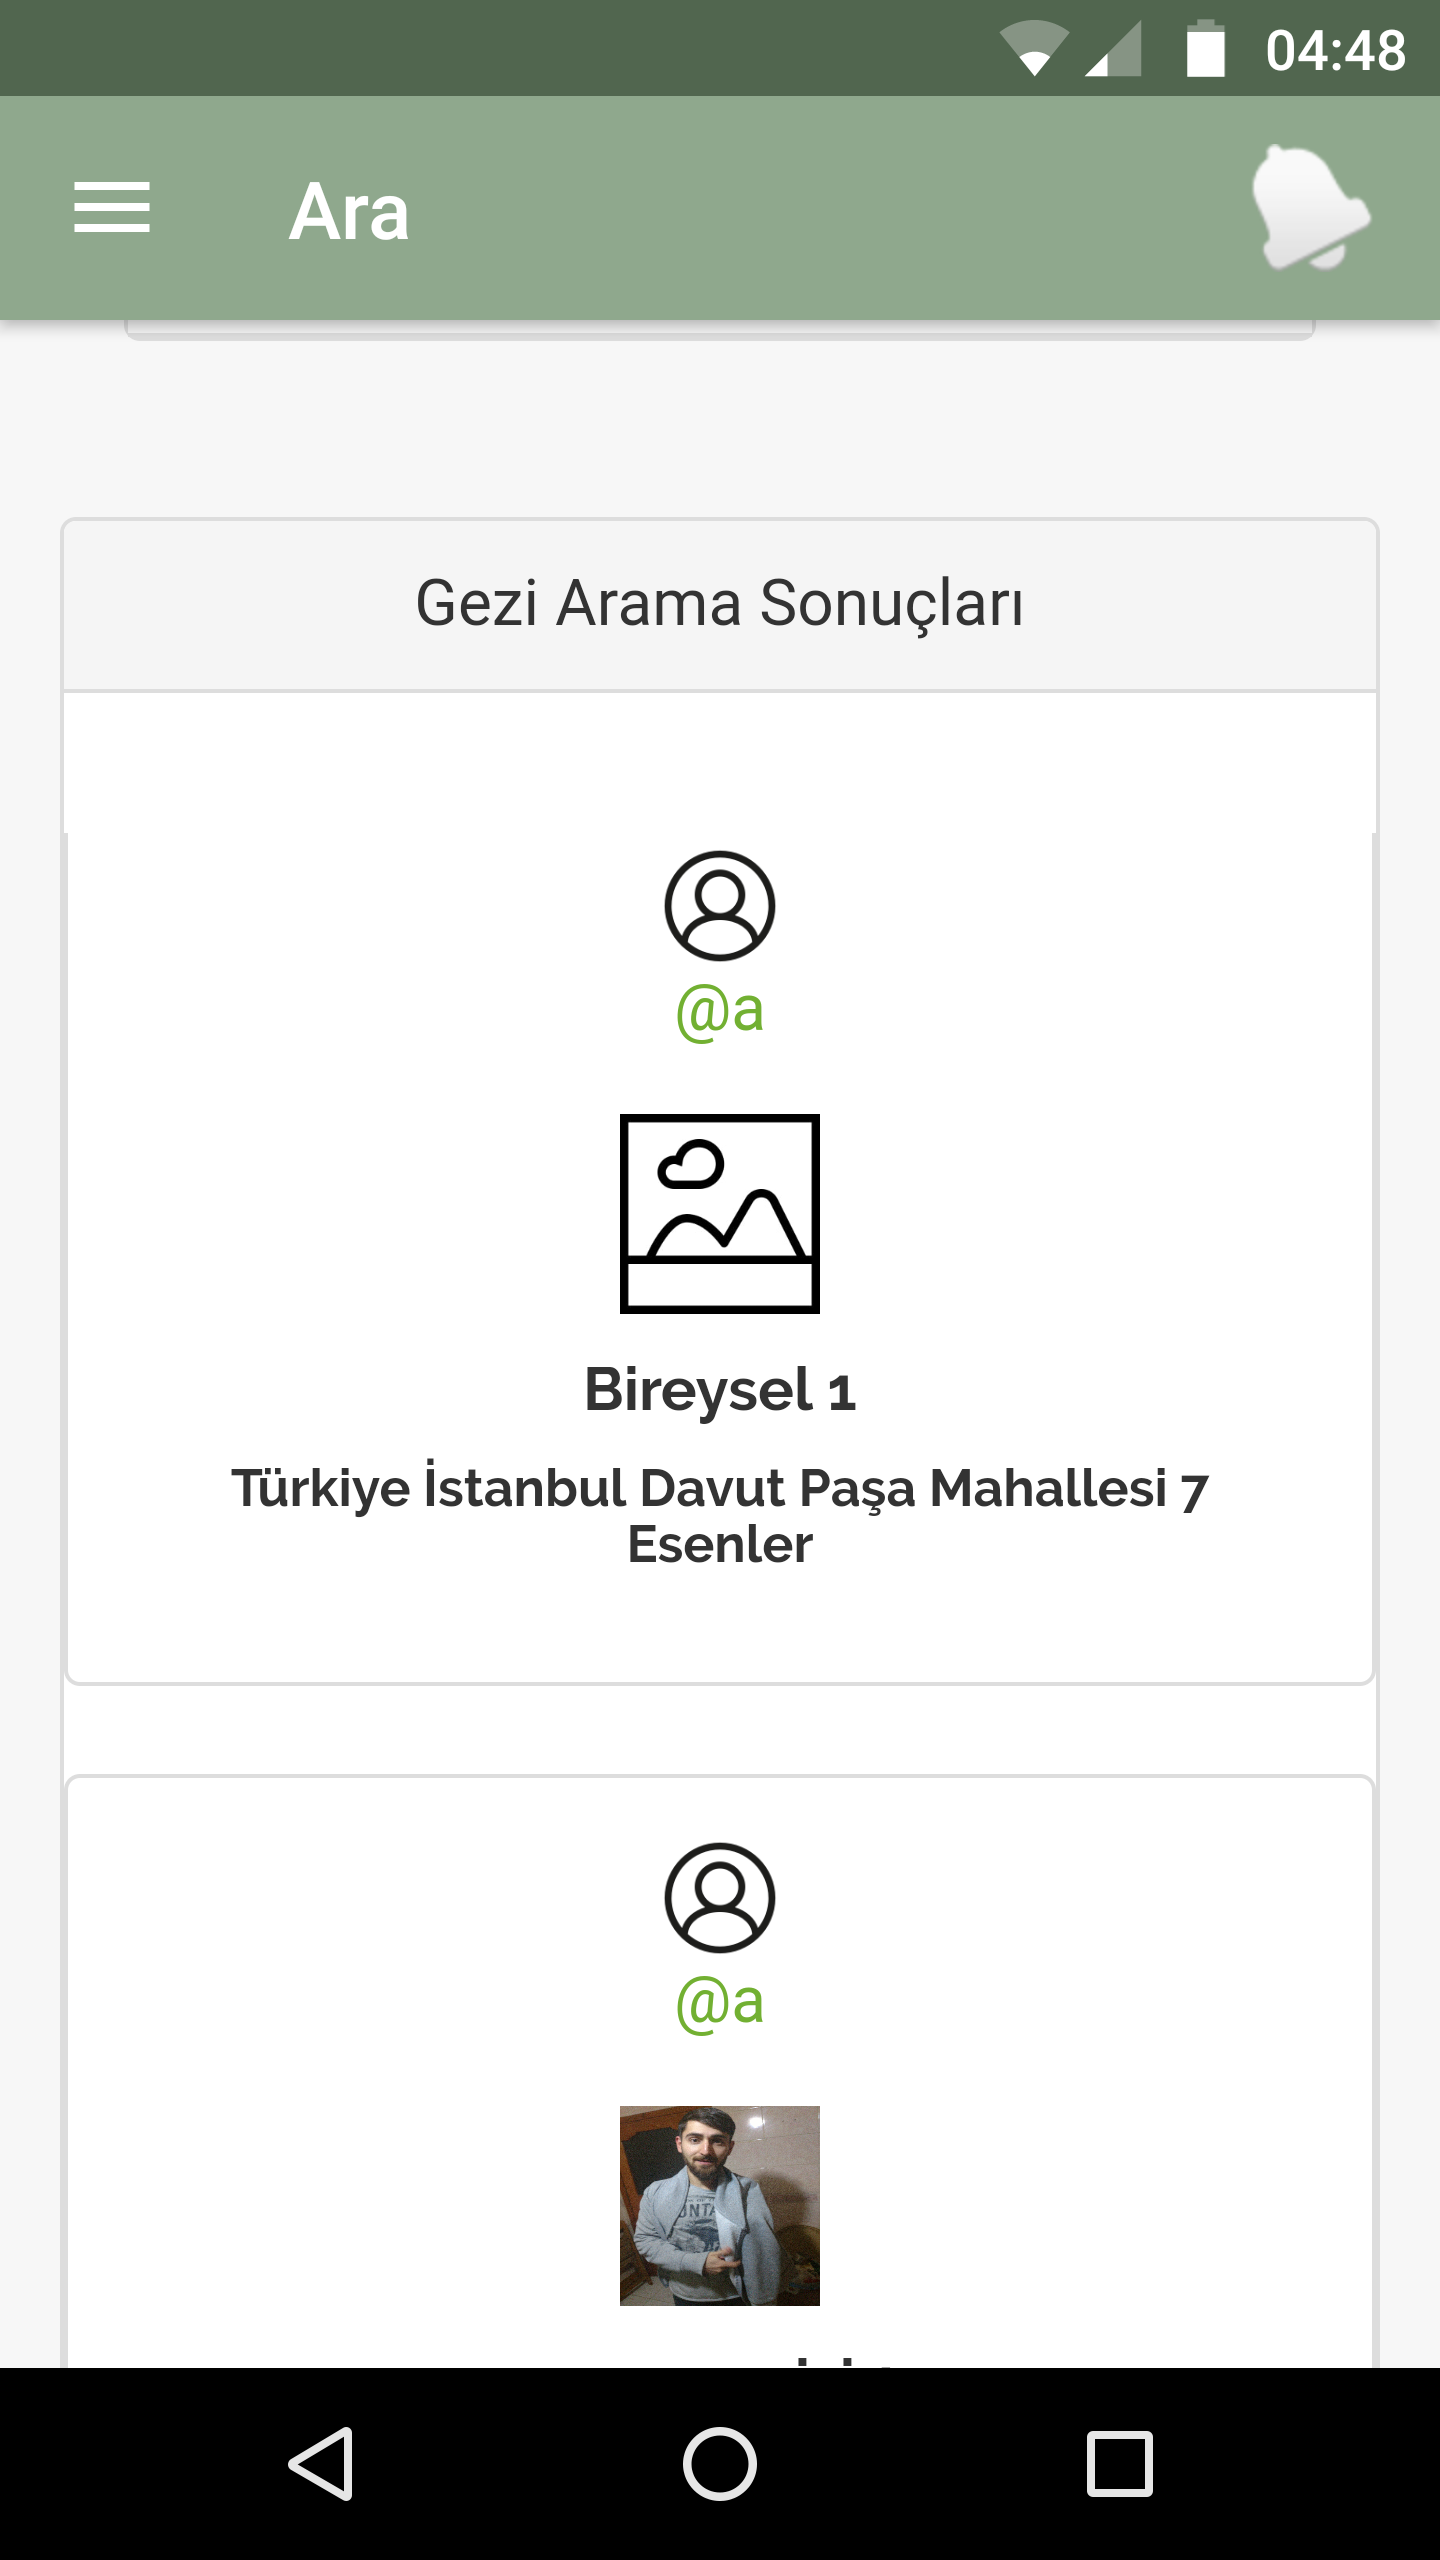
\includegraphics[width=70mm,scale=0.7]{projectChapters/images/mobilGeziArama.png}
\caption{Mobile application search page}
\label{fig:mobilGeziArama}
\end{figure}

\newpage

In mobile application users are able to download trips either from the ones which is shared by their friends or the ones they find in search section. When user click on download text trip will be downloaded to the local storage of mobile application, after downloading it it will be listed in downloaded trips section users can follow the downloaded trip path whenever they want and create a new one by using it. The downloading event is shown in Figure 
\ref{fig:tripDownload}.

\begin{figure}[!htbp]
\centering
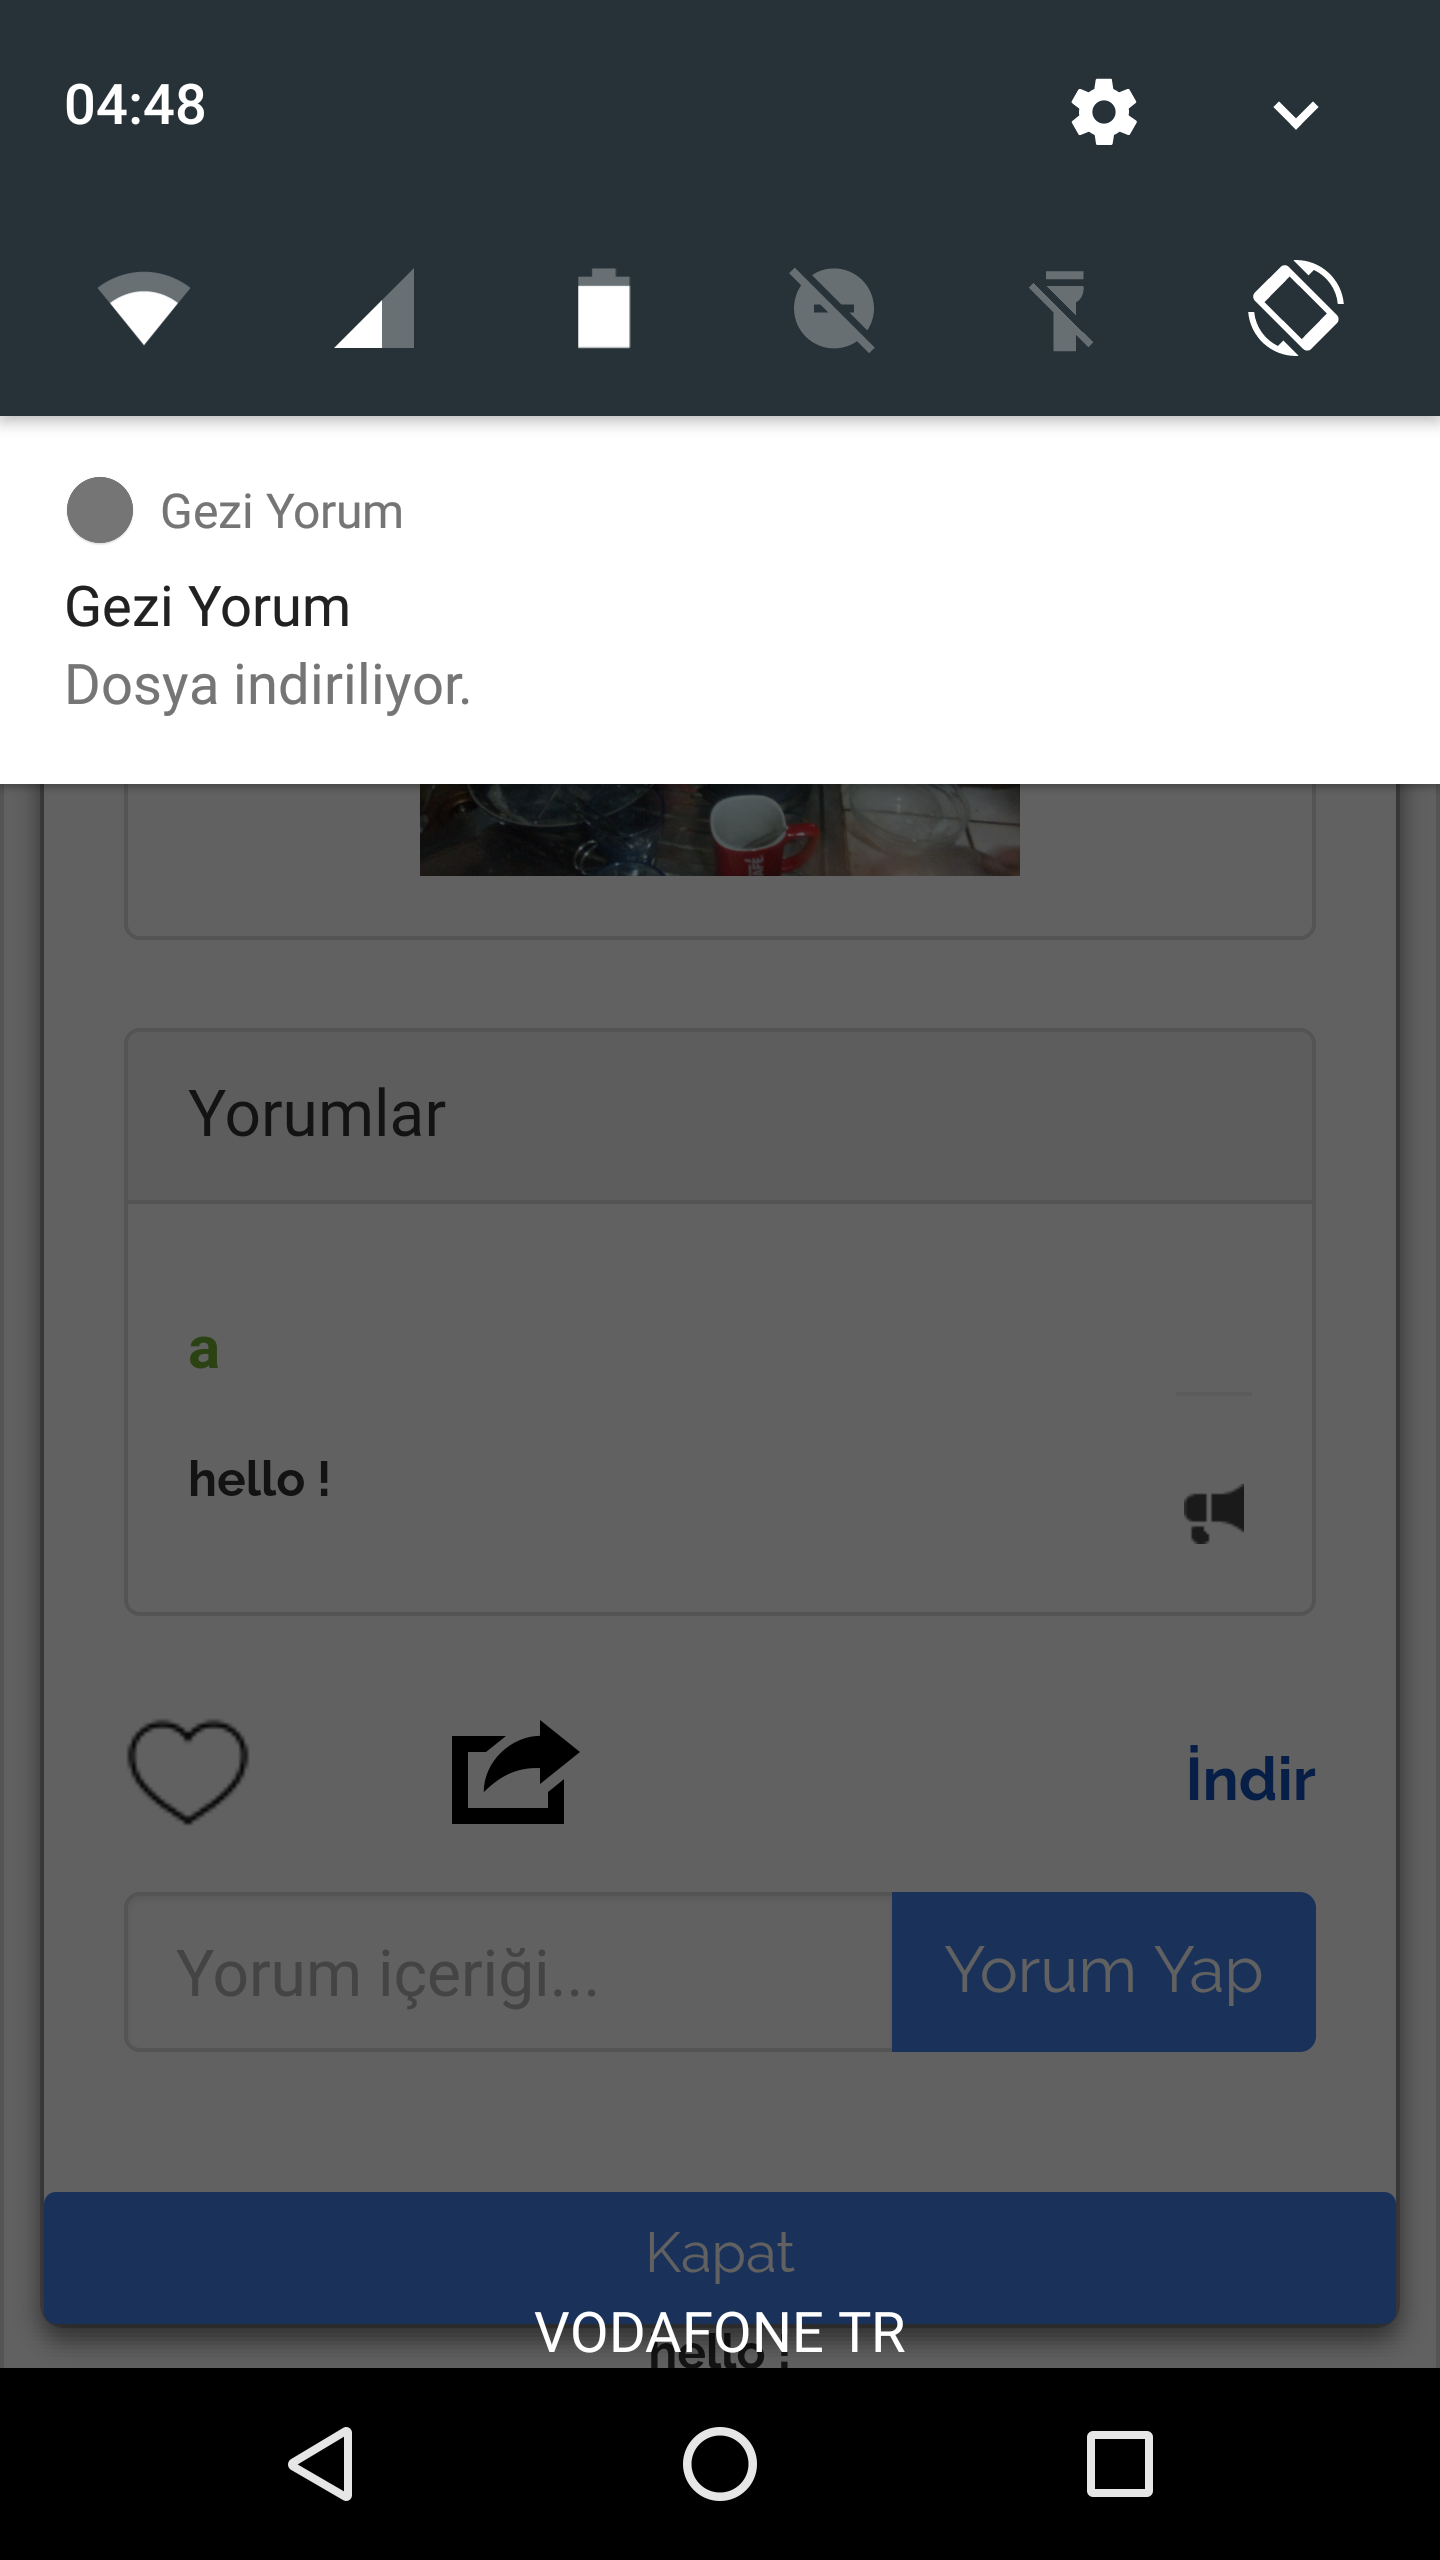
\includegraphics[width=70mm,scale=0.7]{projectChapters/images/tripDownload.png}
\caption{Mobile application trip download module}
\label{fig:tripDownload}
\end{figure}


\newpage

Downloaded trips are shown in the downloaded section, users can see the content of downloaded trip in here. The section is shown in Figure 
\ref{fig:downloadedTrip}.

\begin{figure}[!htbp]
\centering
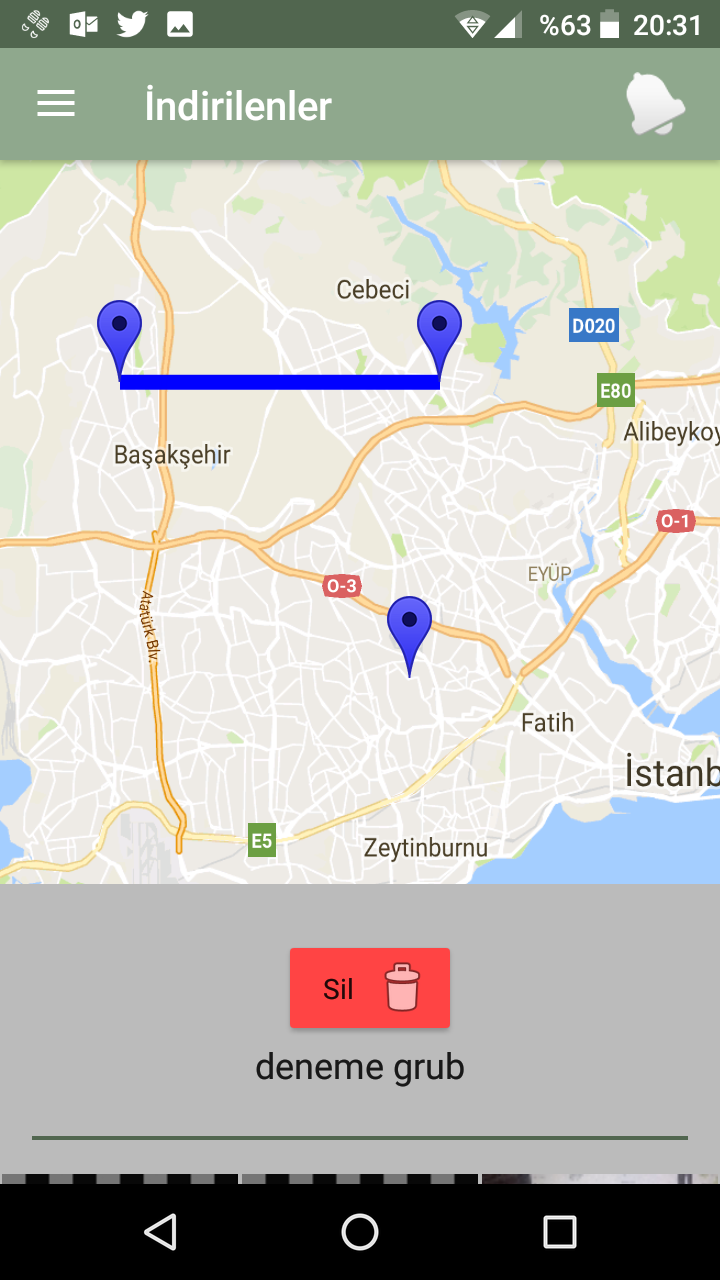
\includegraphics[width=70mm,scale=0.7]{projectChapters/images/downloadedTrip.png}
\caption{Mobile application downloaded trip section}
\label{fig:downloadedTrip}
\end{figure}

\newpage

Users can start a new trip by using downloaded trip which can be a single or group one. If they prefer to create a group trip by that they can create a trip request by adding their friends to   participant list, this section is shown in Figure \ref{fig:downloadedTripManage}.

\begin{figure}[!htbp]
\centering
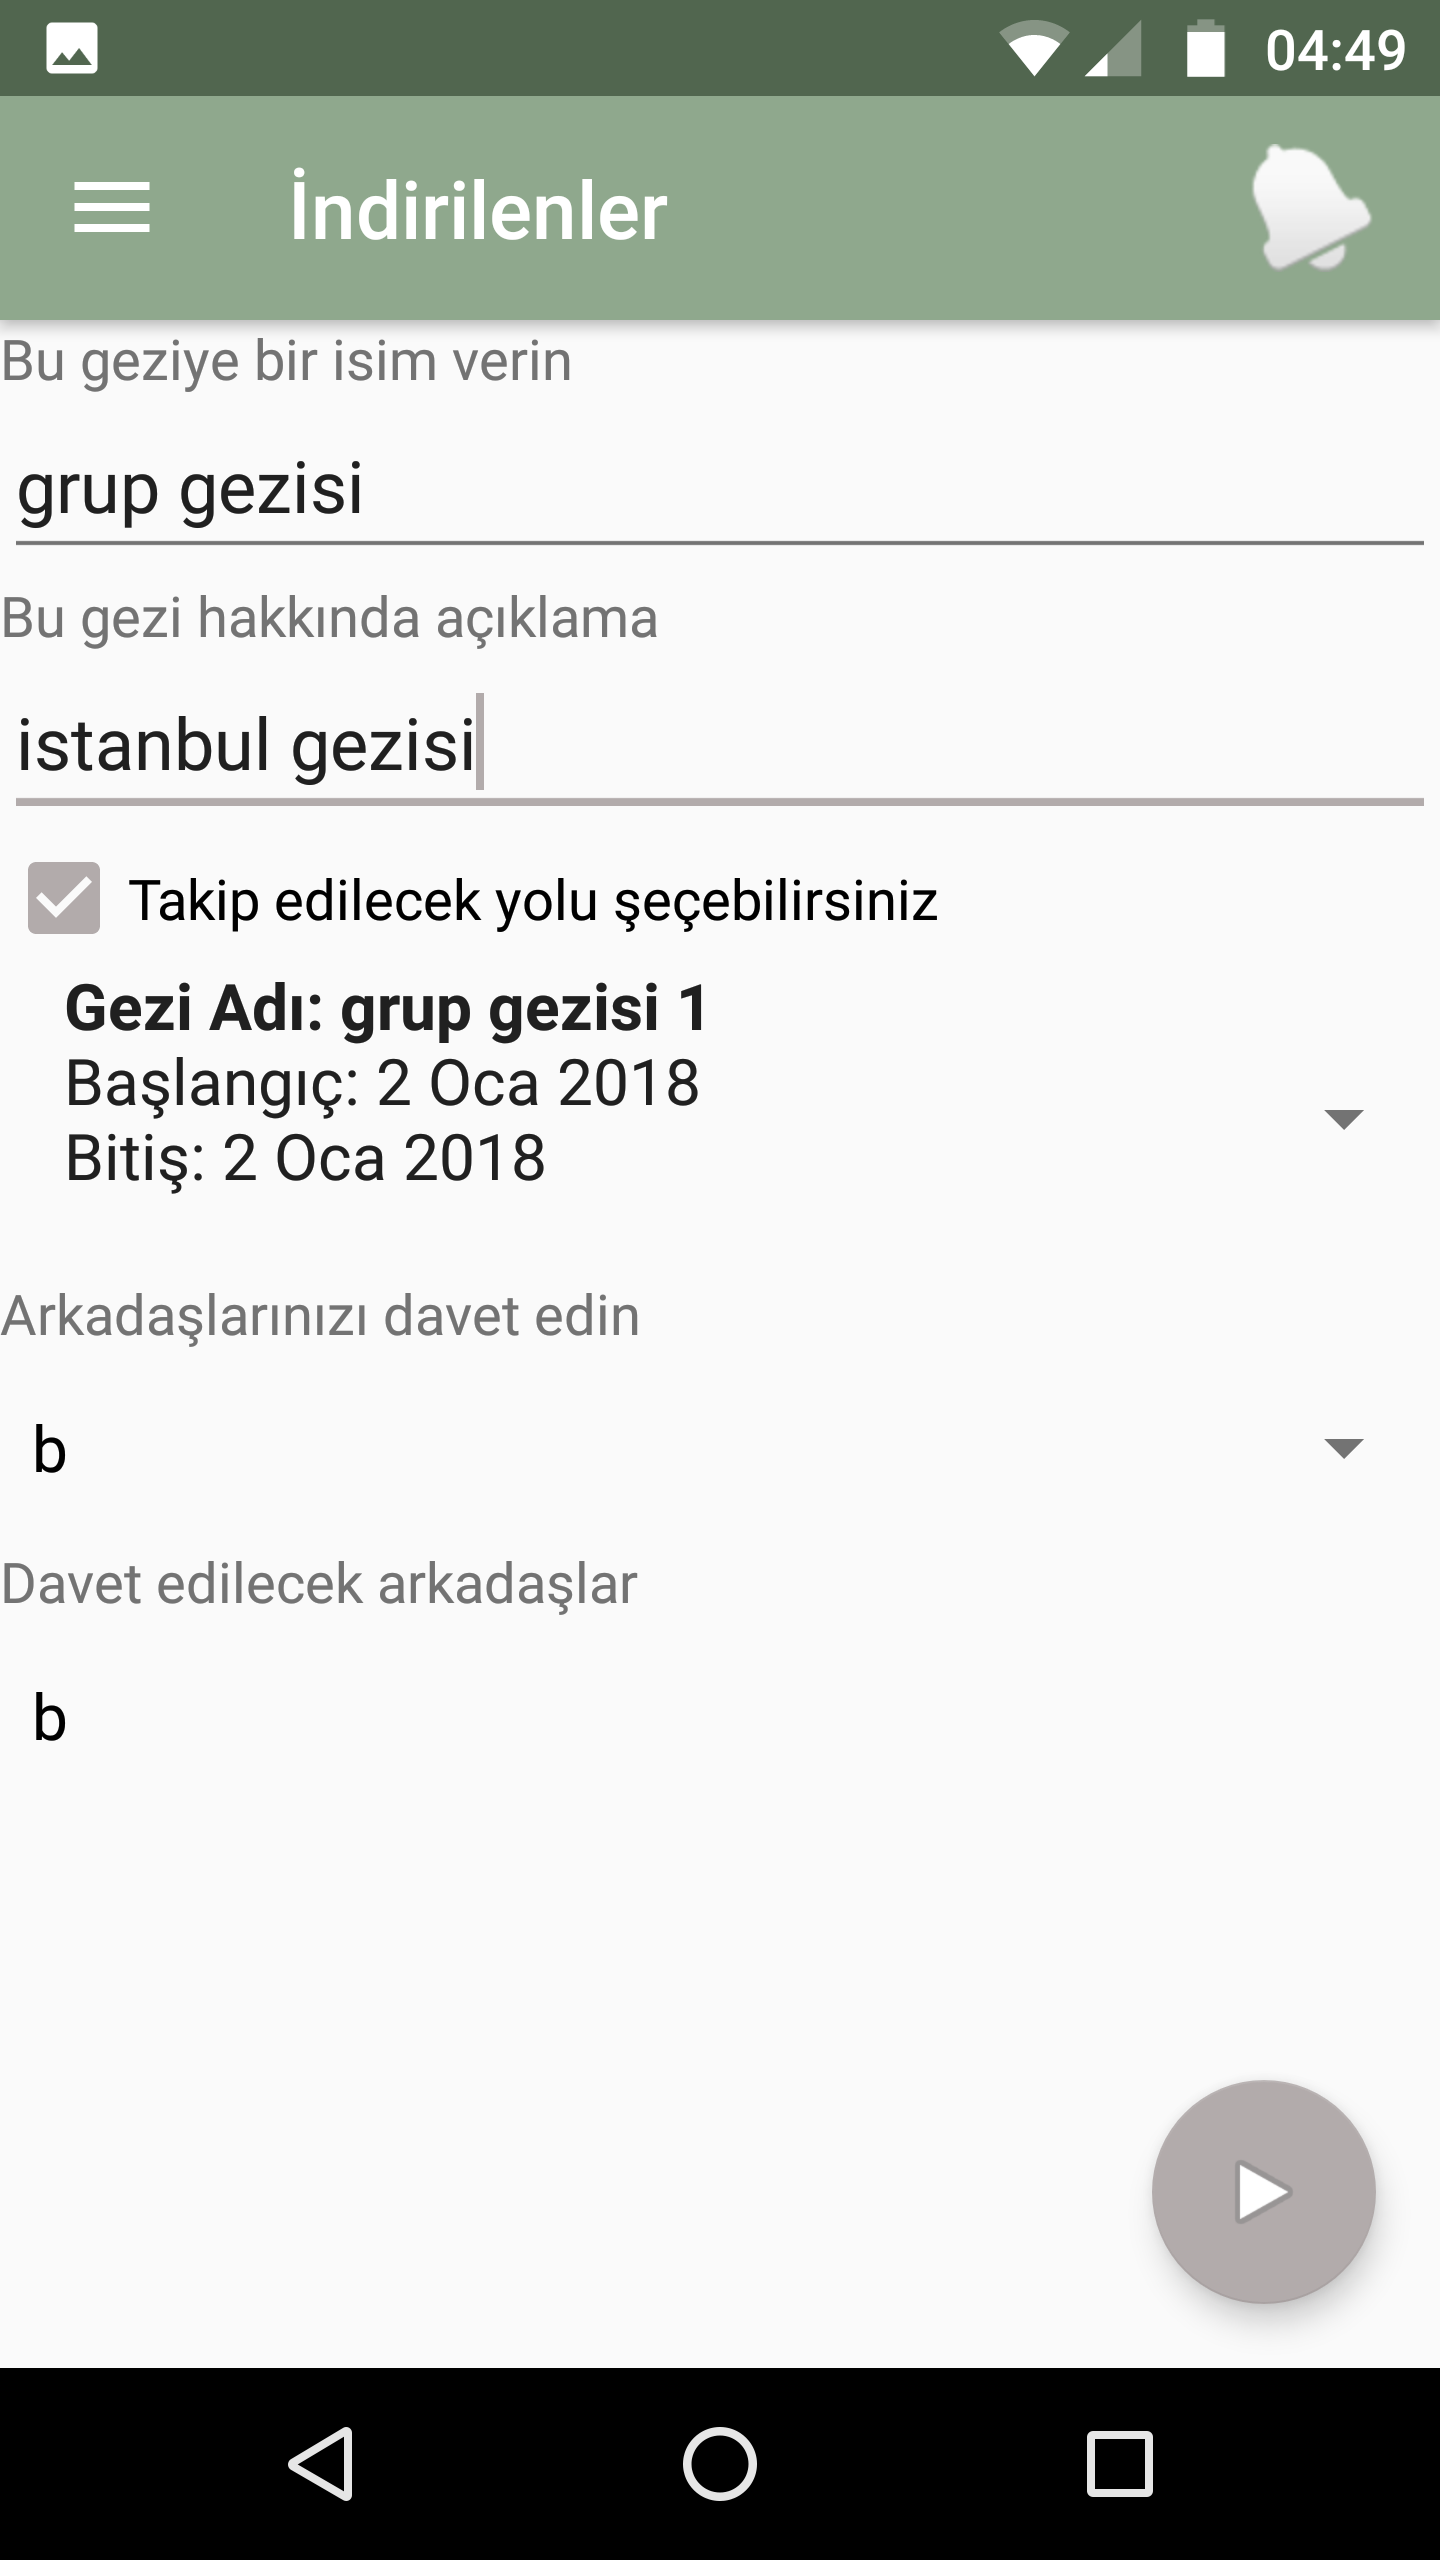
\includegraphics[width=70mm,scale=0.7]{projectChapters/images/downloadedTripManage.png}
\caption{Mobile application downloaded trip section}
\label{fig:downloadedTripManage}
\end{figure}

\newpage

Users can create a trip by using mobile application, poly lines which is the curves on map are generated with tracking the GPS signals of user by the application. If the user following a downloaded trip, downloaded trip's poly line will be different coloured than users own poly line. User can add medias by clicking on little plus sign, then a pop-up is shown. Those pop-ups includes buttons to record audio, to capture picture, or save video footage depending upon the type of the media which user want to save. User can also stops and starts the trip whenever her or she prefers. The section is shown in Figure \ref{fig:tripCreateSection}.

\begin{figure}[!htbp]
\centering
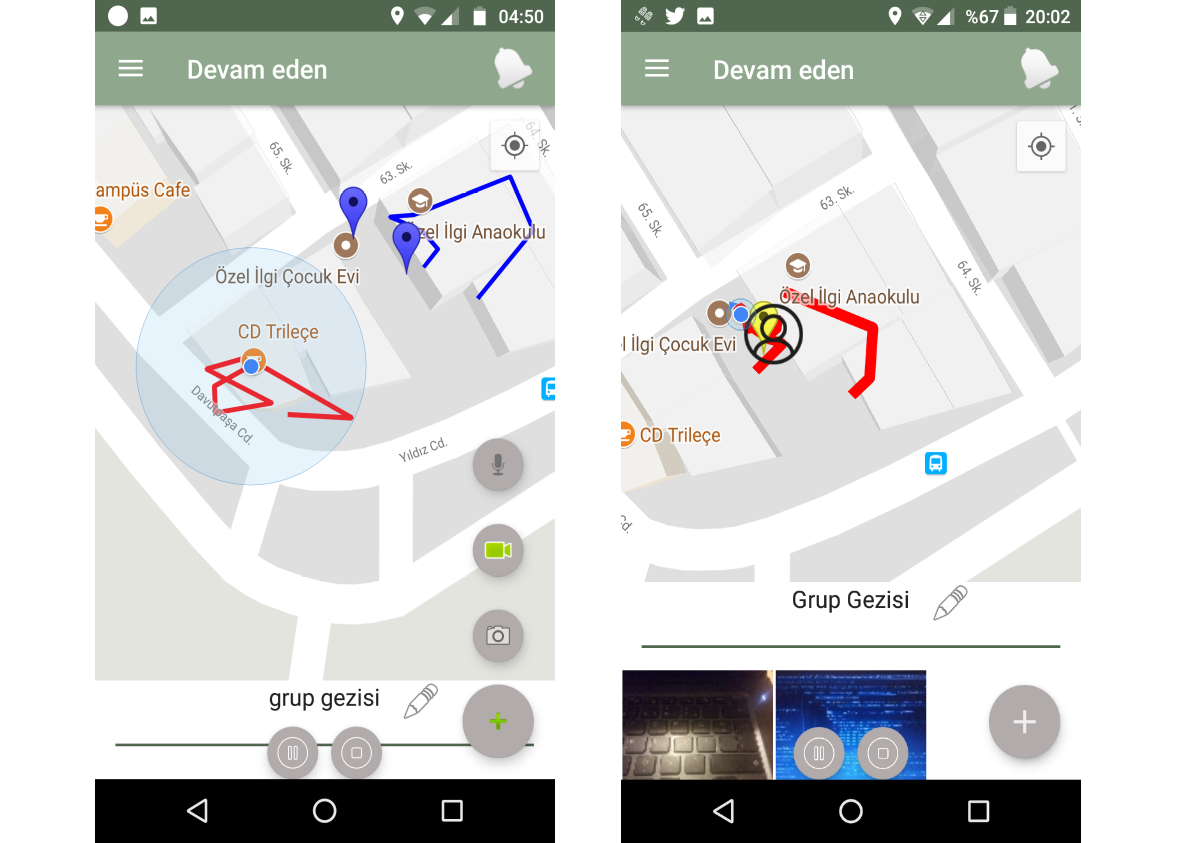
\includegraphics[width=70mm,scale=0.7]{projectChapters/images/tripCreateSection.png}
\caption{Mobile application trip creating module}
\label{fig:tripCreateSection}
\end{figure}

\newpage

By using trip creation module user may want to save some medias, if so those are listed in the created medias section, user evaluate them show them or even delete them if he or she didn't like saved medias. This section is shown in \ref{fig:createdMedias}.

\begin{figure}[!htbp]
\centering
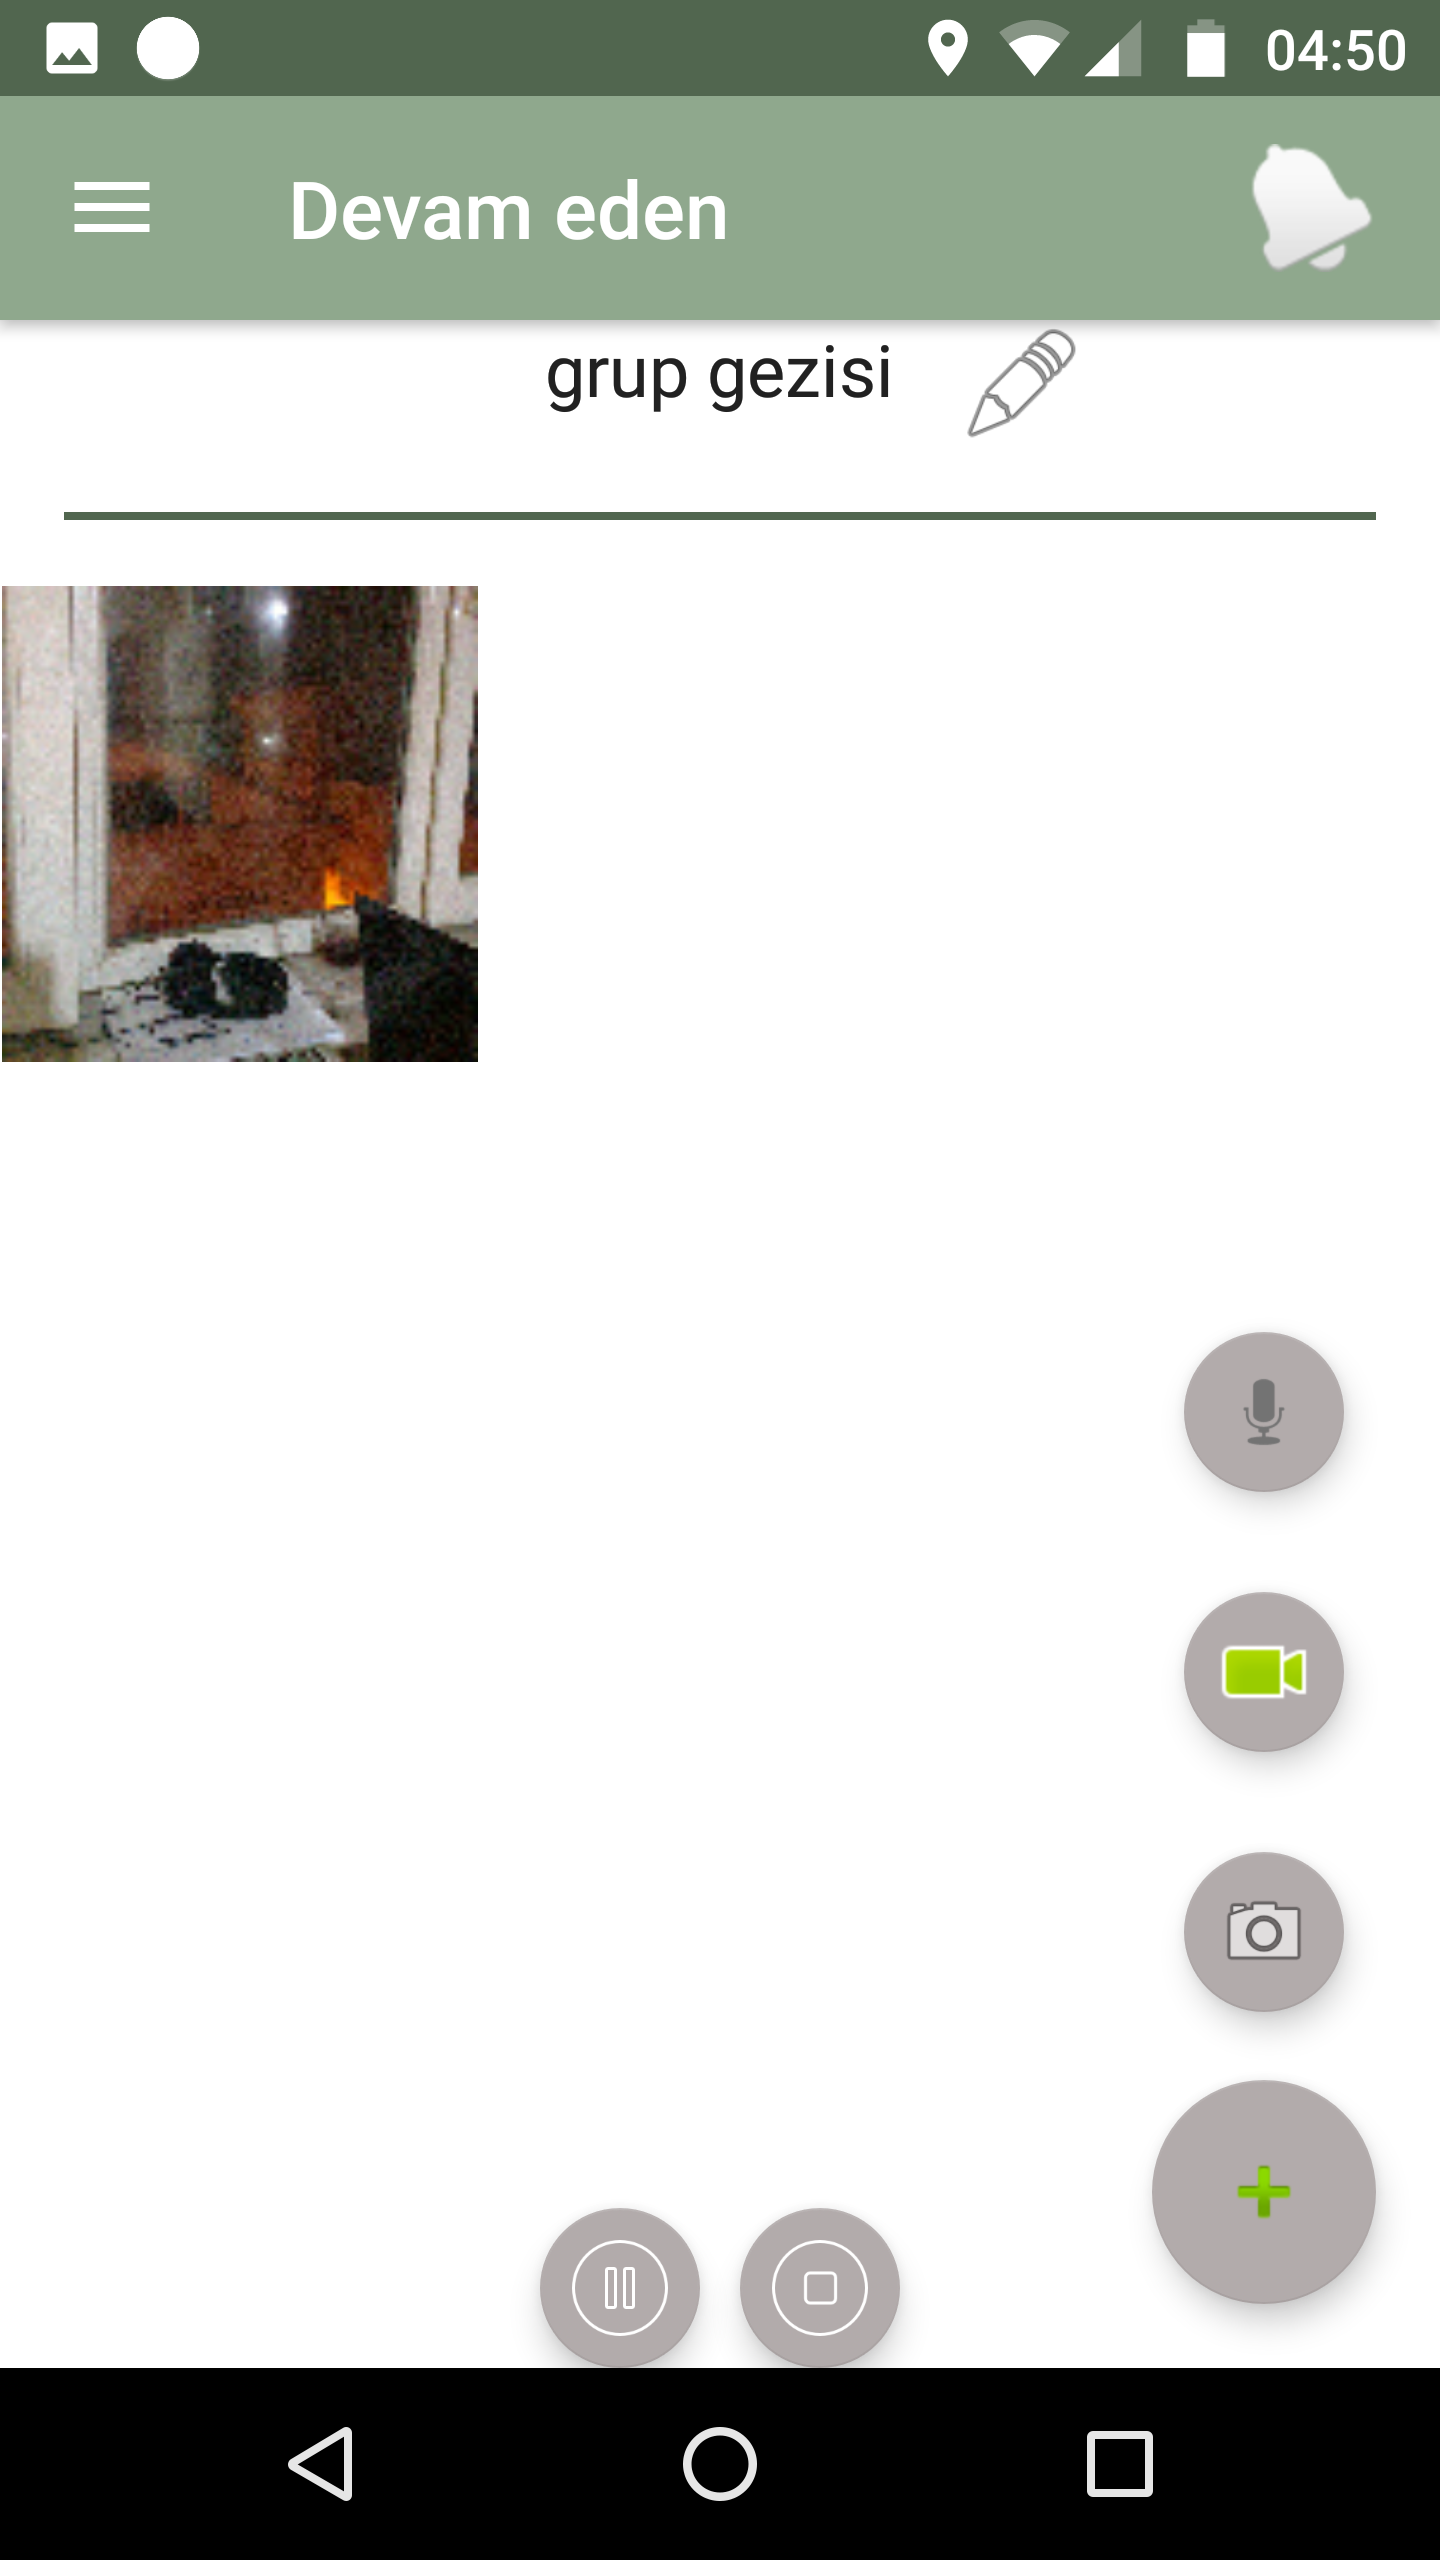
\includegraphics[width=70mm,scale=0.7]{projectChapters/images/createdMedias.png}
\caption{Mobile application trip managing medias while creating trip module}
\label{fig:createdMedias}
\end{figure}



If user finishes trips it will be moved to the timeline section to be evaluated whether it is going to be shared or not. This section is like a review section if they don't want to save the trip after reviewing content users may want to delete or if they like they can share by clicking on the share button. This module is shown in Figure \ref{fig:timeLine}.

\begin{figure}[!htbp]
\centering
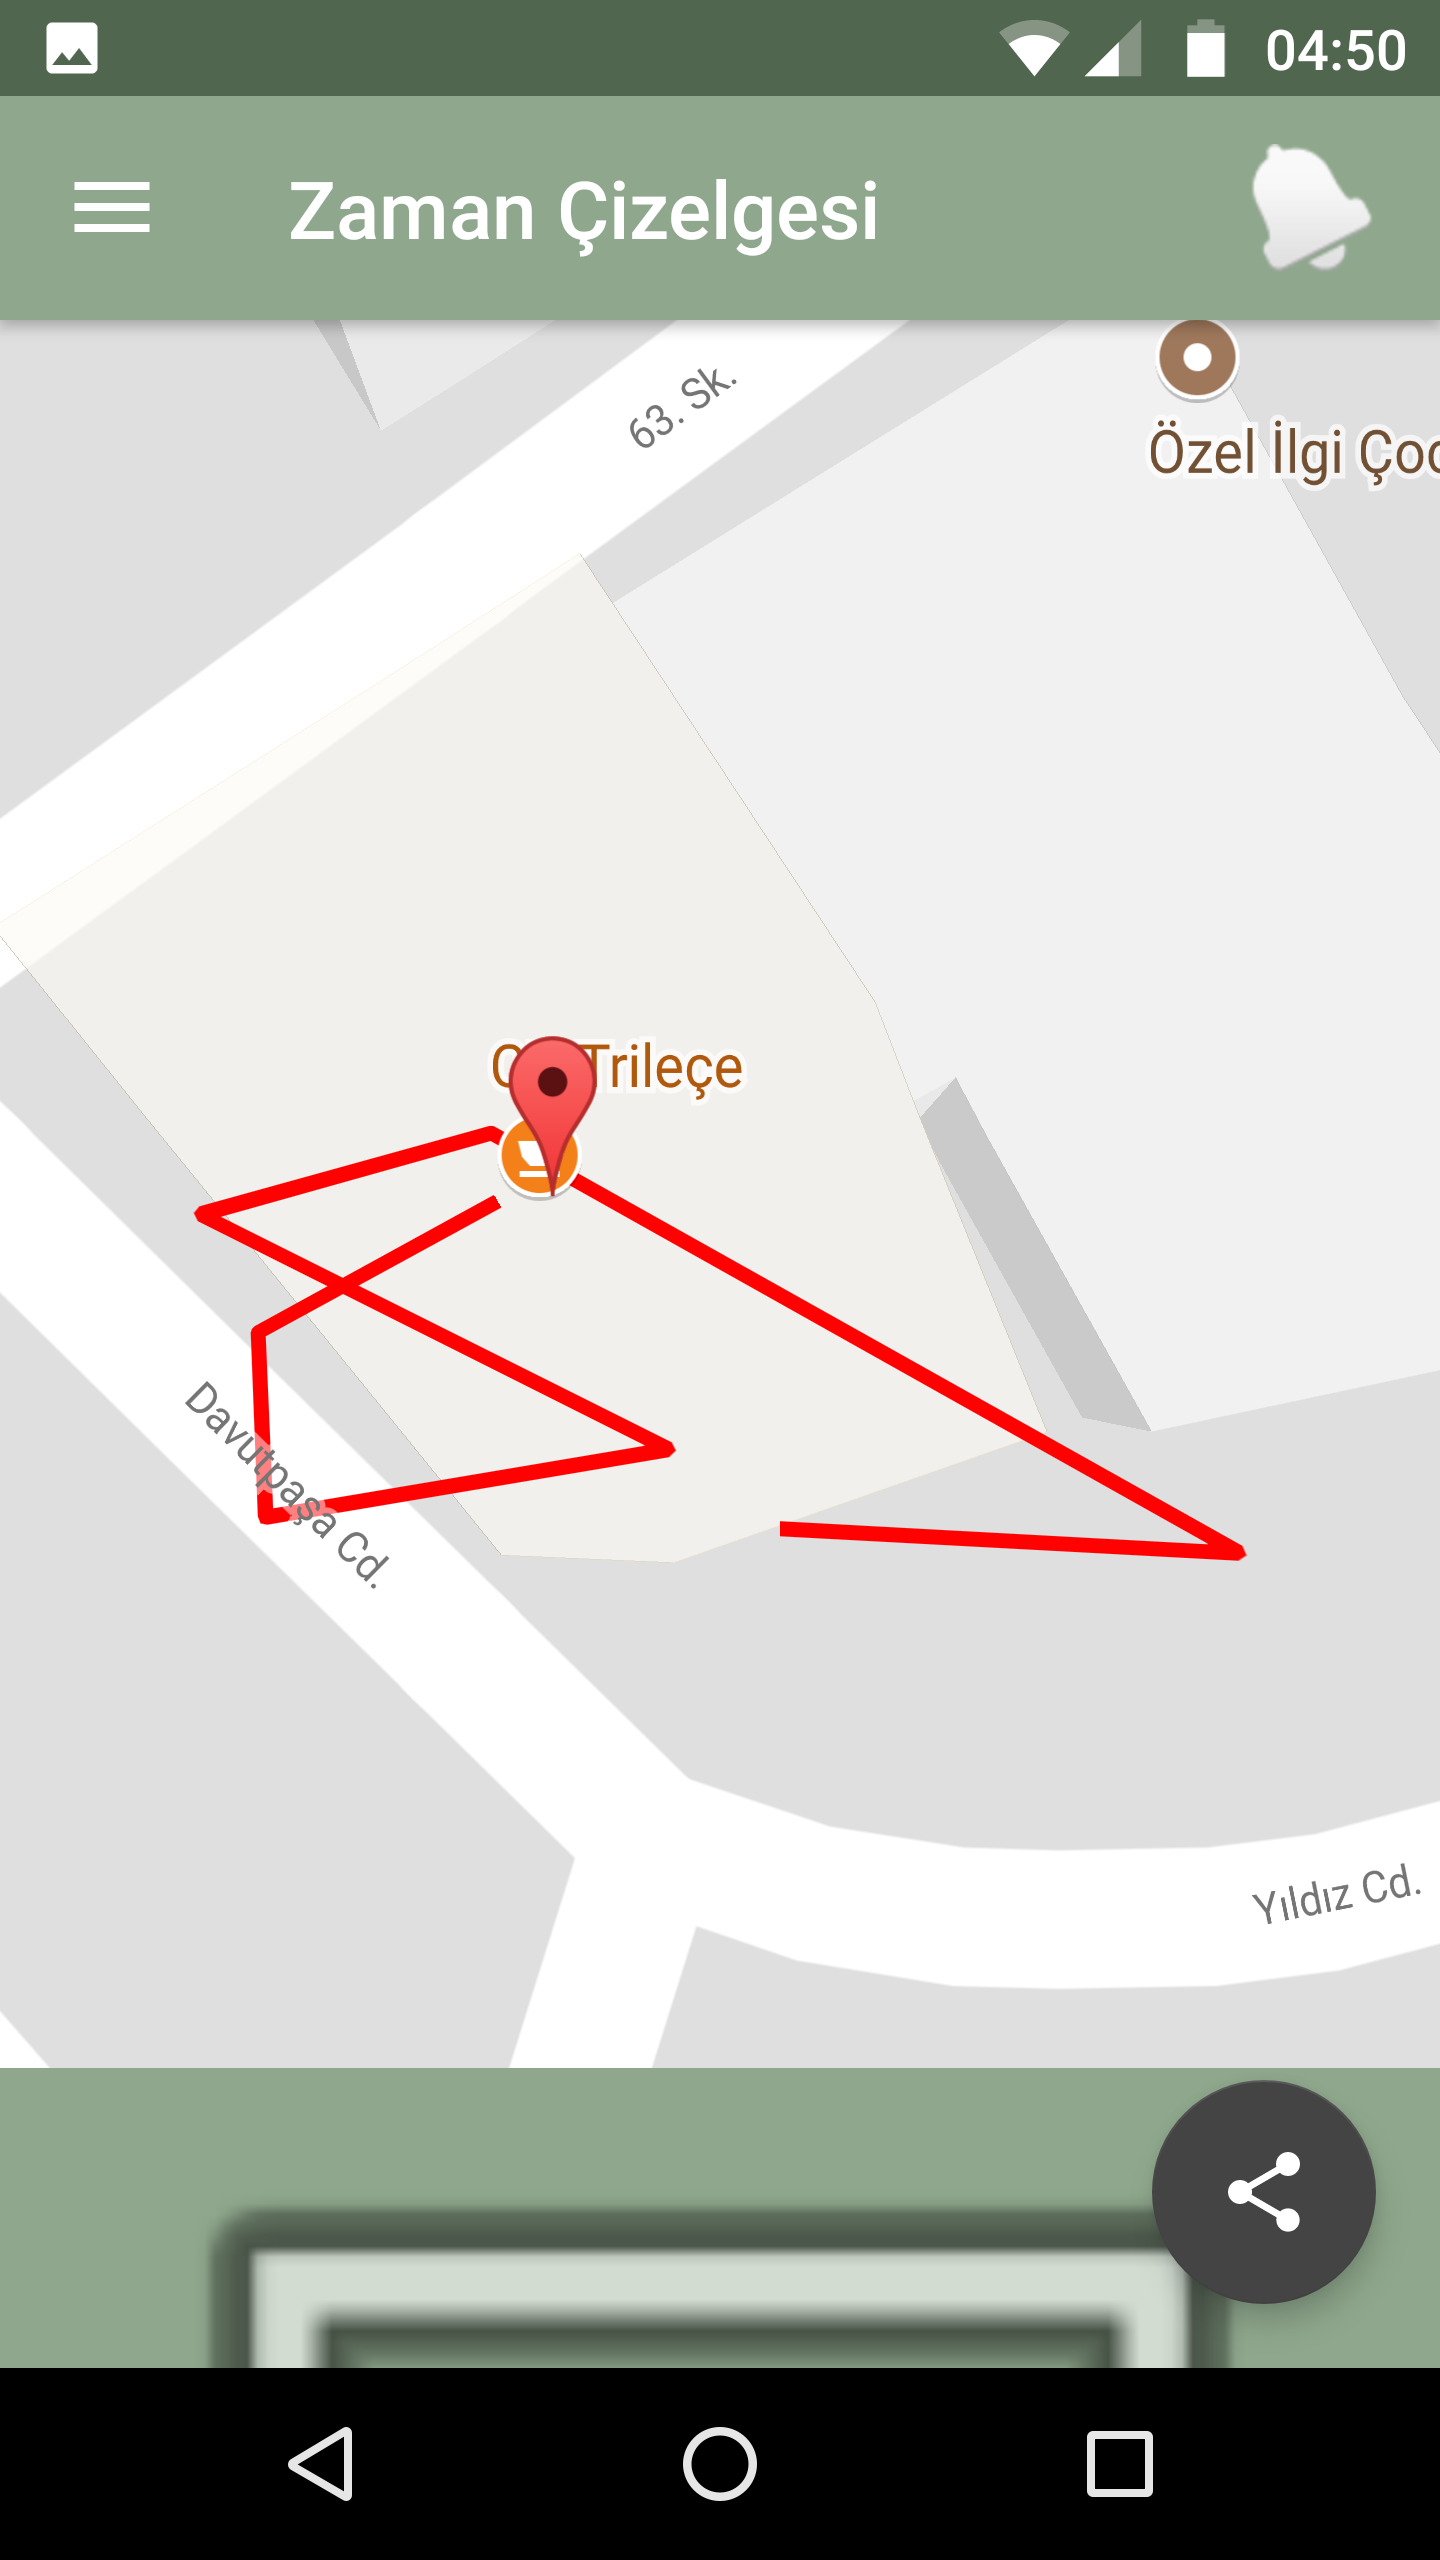
\includegraphics[width=70mm,scale=0.7]{projectChapters/images/timeLine.png}
\caption{Mobile application timeline module}
\label{fig:timeLine}
\end{figure}
 









